%%
%% Copyright 2007, 2008, 2009 Elsevier Ltd
%%
%% This file is part of the 'Elsarticle Bundle'.
%% ---------------------------------------------
%%
%% It may be distributed under the conditions of the LaTeX Project Public
%% License, either version 1.2 of this license or (at your option) any
%% later version.  The latest version of this license is in
%%    http://www.latex-project.org/lppl.txt
%% and version 1.2 or later is part of all distributions of LaTeX
%% version 1999/12/01 or later.
%%
%% The list of all files belonging to the 'Elsarticle Bundle' is
%% given in the file `manifest.txt'.
%%
%% Template article for Elsevier's document class `elsarticle'
%% with harvard style bibliographic references
%% SP 2008/03/01

% \documentclass[preprint,12pt,authoryear]{elsarticle}
\documentclass[final,twocolumn,3p,times,authoryear]{elsarticle}

%% Use the option review to obtain double line spacing
%% \documentclass[authoryear,preprint,review,12pt]{elsarticle}

%% Use the options 1p,twocolumn; 3p; 3p,twocolumn; 5p; or 5p,twocolumn
%% for a journal layout:
%% \documentclass[final,1p,times,authoryear]{elsarticle}
%% \documentclass[final,1p,times,twocolumn,authoryear]{elsarticle}
%% \documentclass[final,3p,times,authoryear]{elsarticle}
%% \documentclass[final,3p,times,twocolumn,authoryear]{elsarticle}
%% \documentclass[final,5p,times,authoryear]{elsarticle}
%% \documentclass[final,5p,times,twocolumn,authoryear]{elsarticle}


%\usepackage{lmodern}
\usepackage[T1]{fontenc}
\usepackage[utf8]{inputenc}


%% For including figures, graphicx.sty has been loaded in
%% elsarticle.cls. If you prefer to use the old commands
%% please give \usepackage{epsfig}

%% The amssymb package provides various useful mathematical symbols
\usepackage{amssymb}
\usepackage{color}
\usepackage{url}
\usepackage{hyperref}
\usepackage{graphicx,array} \graphicspath{{figures/}}
\usepackage{subcaption}
\usepackage{amsmath}
\usepackage{siunitx}
\usepackage{bm}
\usepackage{aasmacros}

\usepackage{enumitem} % to remove when done with todo list

%% The lineno packages adds line numbers. Start line numbering with
%% \begin{linenumbers}, end it with \end{linenumbers}. Or switch it on
%% for the whole article with \linenumbers.
%% \usepackage{lineno}

\newcommand{\nati}[1]{{\color[rgb]{.1,.6,.1}{#1}}}
\newcommand{\todo}[1]{{\color[rgb]{.6,.1,.6}{#1}}}
\newcommand{\assign}[1]{{\color[rgb]{.8,.5,.8}{Assigned: #1 }}}

\newcommand{\figref}[1]{Figure~\ref{fig:#1}}
\newcommand{\tabref}[1]{Table~\ref{tab:#1}}
\newcommand{\secref}[1]{Section~\ref{sec:#1}}
%\newcommand{\secref}[1]{\S\ref{sec:#1}}
\newcommand{\eqnref}[1]{(\ref{eqn:#1})}

\renewcommand{\b}[1]{{\bm{#1}}}   % bold symbol

% MATH SYMBOLS
\newcommand{\1}{\b{1}}              % all-ones vector
\newcommand{\0}{\b{0}}              % all-zero vector
\newcommand{\g}[1]{\b{#1}}
\newcommand{\G}{\mathcal{G}}
\newcommand{\V}{\mathcal{V}}
\newcommand{\E}{\mathcal{E}}
\newcommand{\C}{\mathcal{C}}
\newcommand{\B}{\mathcal{B}}
\renewcommand{\L}{\b{L}}
\newcommand{\tL}{\tilde{\L}}
\newcommand{\W}{\b{W}}
\newcommand{\I}{\b{I}}
\newcommand{\D}{\b{D}}
\newcommand{\U}{\b{U}}
\newcommand{\x}{\b{x}}
\newcommand{\X}{\b{X}}
\newcommand{\y}{\b{y}}
\newcommand{\Y}{\b{Y}}
\newcommand{\bu}{\b{u}}
\newcommand{\f}{\b{f}}
\newcommand{\trans}{^\intercal}
\newcommand{\R}{\mathbb{R}}
\newcommand{\bLambda}{\b{\Lambda}}
\newcommand{\blambda}{\b{\lambda}}
\newcommand{\bO}{\mathcal{O}}
\DeclareMathOperator*{\esp}{E}
\DeclareMathOperator*{\var}{Var}
\DeclareMathOperator*{\vect}{vec}
\DeclareMathOperator*{\argmin}{arg \, min}
\newcommand{\pkg}[1]{\texttt{#1}}


\journal{Astronomy and Computing}

\begin{document}

\begin{frontmatter}

%% Title, authors and addresses

%% use the tnoteref command within \title for footnotes;
%% use the tnotetext command for theassociated footnote;
%% use the fnref command within \author or \address for footnotes;
%% use the fntext command for theassociated footnote;
%% use the corref command within \author for corresponding author footnotes;
%% use the cortext command for theassociated footnote;
%% use the ead command for the email address,
%% and the form \ead[url] for the home page:
%% \title{Title\tnoteref{label1}}
%% \tnotetext[label1]{}
%% \author{Name\corref{cor1}\fnref{label2}}
%% \ead{email address}
%% \ead[url]{home page}
%% \fntext[label2]{}
%% \cortext[cor1]{}
%% \address{Address\fnref{label3}}
%% \fntext[label3]{}

\title{HealpixNet: Efficient spherical Convolutional Neural Network with Healpix sampling for cosmological applications}
% \title{Efficient Spherical ConvNet with Graph Convolutions for Cosmological Applications}
% \title{HealpixNet: Efficient spherical Convolutional Neural Network with graphs and Healpix sampling for cosmological applications}
%\title{HealpixNet: Graph Convolutional Neural Network for efficient spherical convolutions on Healpix sampling for cosmological applications}
% Graph Convolutional Networks for efficient spherical ???
% Efficient spherical ??? with GCNs and Healpix sampling
% (Tomek) How about HealpixCNN? Or HealpixNet? Or HealNet?}
% spherical convolutions with graphs

%% use optional labels to link authors explicitly to addresses:
%% \author[label1,label2]{}
%% \address[label1]{}
%% \address[label2]{}

\author{}

\address{}

\begin{abstract}

%Convolutional Neural Networks (CNNs) are becoming an important analysis tool in cosmology and astrophysics.
% Michaël: useful info? To me this is not an argument for our approach. Maybe we have to expand it?

% Architectures are then designed similarly to the classical CNNs used for image analysis.
% HealpixCNN (???) uses Tensorflow as the underlying engine and can utilize most of it functionalities.
% Michaël: not relevant for the abstract in my opinion

Convolutional Neural Networks (CNNs) are now a cornerstone of the Deep Learning toolbox and have led to many breakthroughs in Artificial Intelligence.
So far, these networks have mostly been developed for regular Euclidean domains such as those supporting images, audio, or video.
Because of their success, CNN-based methods are becoming increasingly popular in Cosmology.
Nevertheless, cosmological data often comes in a form of spherical maps, which makes the use of traditional CNNs impractical and complicated.
Typically, the spherical format for spherical maps is HEALPix, which uses an equal-area, isolatitude sampling.
As a response to this gap, we present a spherical CNN for analysis of full and partial HEALPix maps, which we call HealpixNet.
We construct a spherical CNNs by representing the sphere as a graph.
Graphs are versatile data structures which can represent pairwise relationships between objects or act as a discrete representation of a continuous manifold.
Leveraging the graph, we define many of the standard CNN operations, such as convolution and pooling, with the filters restricted to being radial.
HealpixNet is a special case of a graph CNN, tailored to the HEALPix sampling of the sphere.
% TBD if we include it
% This approach is computationally more efficient than using spherical harmonics to perform convolutions, an alternative that has been explored previously.
We demonstrate the method on a classification problem of mass maps from two cosmological models and compare the performance of the CNN with that of two baseline classifiers, based on the power spectrum and pixel density histogram.
Our experimental result show that the performance of HealpixNet to always better or equal to both of these baselines.
For high noise levels and for data covering only a smaller fraction of the sphere, HealpixNet achieves typically 10\% better classification accuracy than those baselines.
Finally, we propose a visualization of filters learned by the HealpixNet from the mass maps as some analysis tool for the neural network.
Code and examples are available at \todo{\url{https://github.com/SwissDataScienceCenter/HealpixNet}}.

%As a response to that fact, we are witnessing an increasing interest in the generalization of CNNs to graphs.
% Graphs are versatile data structures which can represent pairwise relationships between objects or act as a discrete representation of a continuous manifold.
% In this paper we take the latter view and represent a sampled sphere as a graph, for which we define the convolution and pooling operations.
% Spherical maps appear in many applications, such as the study of phenomena on the Earth for meteorologists or on the sky for cosmologists.
% A popular format for spherical maps is Healpix, which uses an equal-area, isolatitude sampling.
% Hence, we present a spherical CNN for analysis of full and partial Healpix maps, which we call HealpixNet.
% \nati{I am not that we should talk about pooling in the abstract. Another angle would be to say that HEALPix sampling is well suited for spherical CNN with graphs as a) it is very regular => the graph capture well the spherical structure of the Manifold and b) pooling is natural.}
% While the convolution on arbitrary graphs has mostly been sorted out, a general pooling operation has not been discovered so far.
% As such, while HealpixNet is a special case of a graph CNN, it is tailored to the Healpix sampling of the sphere.
% This approach is computationally much more efficient than using spherical harmonics to perform convolutions, an alternative that has been explored previously.
% The filters learned by the HealpixNet are restricted to being radial.
% Michaël: not necessary in the abstract?
% We demonstrate the method on a classification problem of mass maps from two cosmological models.
% \nati{Should we specify what are the baselines? I think not.}
% A standard benchmark for that problem is to train an SVM on the histograms of map pixel values. Another is to use the power spectral density instead.
% HealpixNet achieves \todo{xx\%} better accuracy than those baselines, is more robust to noise, and is \todo{faster?}.
% Code and examples are available at \todo{\url{https://github.com/xxx}}.
\end{abstract}

\begin{keyword}
Spherical Convolutional Neural Network \sep
HealpixNet \sep
Graph CNN \sep
Cosmological data analysis \sep
Mass mapping
\end{keyword}

\end{frontmatter}

%% \linenumbers

\section{TODO list}
\begin{itemize}[noitemsep,topsep=0pt,parsep=0pt,partopsep=0pt]
    \item (NP) Figures  A.15, 6, 5
    \item (TK) add small description of maps\_downsampled\_64.npz in the whole\_sphere notebook.
    \item (TK) update the README for data zip - file from NP
    \item (NP) Finalise readme on Github code
    \item (Waiting for Zenodo) (NP) Finalize the data on zenodo
    \item TK check part sphere notebook and whole sphere
    \item branch with notebooks with plots (results) NP
    \item Michael section 4.5 (efficient convolutions) and 3.2 (conv on graphs)
    \item NP move the repo to HealpixNet
	\item check if papers which appear as arxiv were not published in a conference or journal
    \item (TK) add info on comparison with histograms, so that it's just a demonstration
    \item (TK NP) if we have time make a new candidate for network plot (optional)
    \item (first version done) conclusions
    \item Should the heat example go to appendix?
    \item TK read the heat section again
    \item TK read the result section
    \item TK check the appendix
    \item TK optional - example of data (CMB (mask) + mass map + radio intensity)
    \item TK read everything
	\item MD add irregular (random) sampling to comparison with spherical harmonics? Could motivate people to think about different samplings.
	\item uniformize text size in figures
\end{itemize}

\begin{figure*}
	\centering
    % 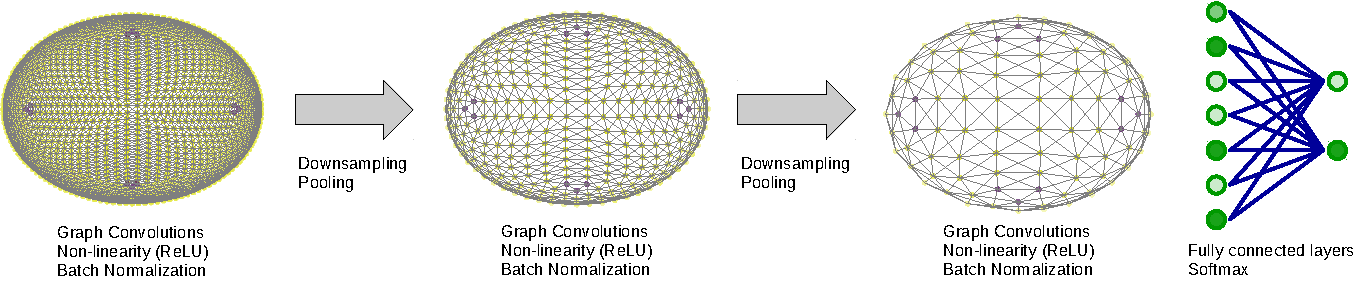
\includegraphics[width=\linewidth]{architecture}
	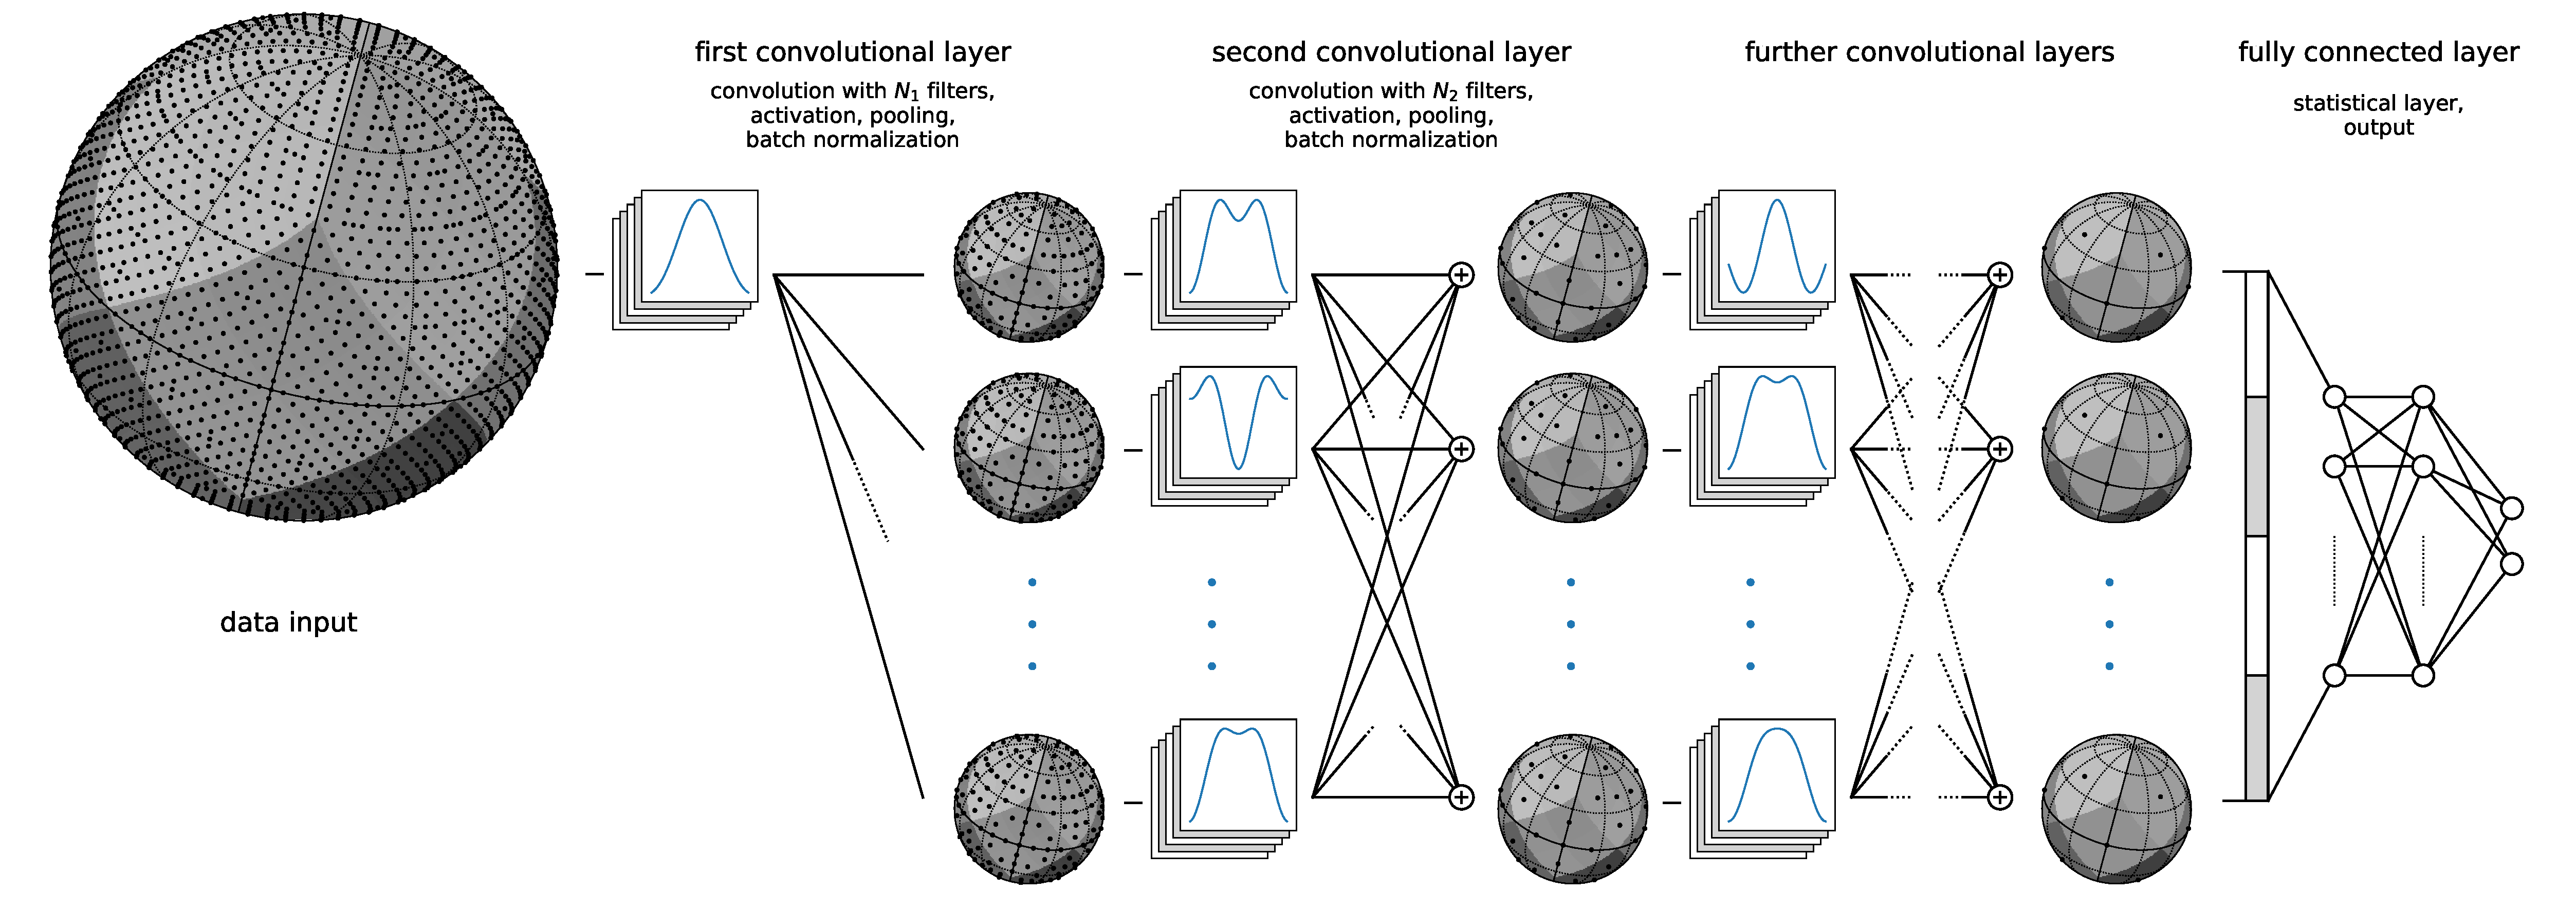
\includegraphics[width=\linewidth]{figure_architecture_v2}
	\caption{Overall network architecture, showing here two convolutional layers acting as feature extractors followed by a fully connected layer with softmax acting as the classifier. \nati{add the stat layer?} A convolutional layer is based on five operations: convolution, non-linearity, batch normalization, down-sampling, and pooling. While most operations are agnostic to the data domain, the convolution and the down-sampling have to be adapted. In this paper, we propose first to model the sphere with a graph and to perform the convolution on the graph. Graphs are versatile data structures which can model any sampling, even irregular or partial. Second, we propose to exploit a hierarchical pixelization of the sphere for the pooling operation. It allows the network to analyze the data at multiple scales while preserving the spatial localization of features. This figure shows a network which operates on the whole sphere. The process is however the same when working with parts of sphere, except that the graph is only built for the part of interest.}
	\label{fig:architecture}
\end{figure*}

\section{Introduction}
\label{sec:intro}

%\subsection{Motivation}

Cosmological and astrophysical data often comes in the form of spherical sky maps.
Observables that cover large parts of the sky, such as the Cosmic Microwave Background (CMB) \citep{planck2015cosmologicalparameters,komatsu2011sevenyear,staggs2018recentdiscoveries}, neutral hydrogen \citep{santos2015cosmologySKA,HI4PI2016fullskyHI}, galaxy clustering \citep{alam2017clusteringgalaxies}, gravitational lensing \citep{troxel2017darkenergy,hildebrandt2017kidscosmological}, and others, have been used to constrain cosmological and astrophysical models. Deep Learning has recently gained popularity as an analysis tool in cosmology \citep{schmelze2017cosmologicalmodel,luciesmith2018machinelearning,gupta2018nongaussianinformation,gillet2018deeplearning,hassan2018reionizationmodels,aragoncalvo2018classyfyinglarge,ciuca2017cnnstring}, thanks to its ability to capture complicated, non-linear patterns which are often present in the data. Convolutional Neural Networks (CNNs) are particularly well suited for analysis of cosmological data due to the translation invariance built into their architecture. Indeed, sky maps are translation invariant, which means that translating and rotating maps on the sphere doesn't change their interpretation. Only the statistics of the maps is relevant. The location of the map on the sky is always fixed (by where the telescope was looking), and most of the models tested are homogeneous and isotropic (the cosmological principle). As such, learned weights can be shared across the sphere: the network does not have to relearn to detect objects or features at every spatial location.

For cosmological observations it is often the case that the data covers only a part of the sphere.
For ground-based observations this can be due to limited visibility of the sky from a particular telescope location and survey strategy, and for space-based imagers due to masking of the galactic plane area.


% \todo{@Tomek: can you explain why we care about parts of the sphere? (that is an advantage of the graph model over the spherical harmonics)}
% \todo{@Tomek: How is the data acquired? Do telescopes and satellites take measurements according to the HEALPix sampling? (it is also an advantage of our method to be agnostic to the sampling, which might be useful to researchers working with missing data or different models)}
% \nati{@Tomek: I think what Michael has in mind is that the graph approach is very versatile and extendable. It can be used with other samplings (even irregular ones) or only part of the sphere. This flexibility might be an advantage to mention. In particular, compared to~\citet{cohen2018spherical} it allows us to do only do the required computation when only a part of the sphere is considered.}

So far these algorithms have mostly been demonstrated on Euclidean domains, such as flat images.
As such, perhaps the most straightforward approach to the analysis of spherical data is to divide it into small chunks and project those on flat 2D surfaces.
While this mostly works, as demonstrated by \citep{fluri2018deep,gupta2018nongaussianinformation,schmelze2017cosmologicalmodel,gillet2018deeplearning}, it may be more natural for some applications and accurate to work directly on the sphere.
The main challenge in designing a CNN on the sphere is to define a convolution which is suitable to this irregularly sampled domain.

% cohen2017convolutional (ICML workshop) and cohen2018spherical (ICLR best paper) are redundant
A first attempt to generalize CNNs to spherical data was to apply a standard 2D CNN to a grid discretization of the sphere~\citep{boomsma2017spherical}. While this approach leverages the well-developed 2D convolution and hierarchical pooling, it is restricted to those specific grid samplings which are highly irregular on the sphere.
A second attempt by~\citet{cohen2018spherical} was to leverage the spherical Fourier transform and to perform the convolution in the spectral domain, thanks to the convolution theorem. While there exists fast spherical Fourier transforms for some samplings, this approach is still computationally expensive (see \figref{filtering_speed}).
Finally, the use of a graph to model the discretized sphere was considered by~\citet{khasanova2017graphomni} as well, towards the goal of building invariances in the network. While their architecture is fully invariant to translation and rotation on the sphere, they did not take advantage of a hierarchical pixelization of the sphere, and the statistical layer used to be invariant needs to be hand-crafted to capture statistics of interest.

To overcome those shortcomings, we introduce an efficient spherical CNN formulation which uses (i) convolutions on graphs and (ii) hierarchical pooling. The main idea is to represent the sphere $S^2$, a 2-dimensional manifold embedded in $\mathbb{R}^3$, as a graph of connected pixels. The length (or weight) of the shortest path between two pixels is an approximation of the geodesic distance between them on the manifold.
This contribution leverages the emerging field of graph signal processing which defines fundamental signal processing tools such as the Fourier transform for signals defined on graphs \citep{shuman2013emerging}.
Our approach uses the graph CNN formulation introduced by \citet{defferrard2016convolutional}, which is efficient and can adapt to any sampling of the sphere. Using a $k$-nearest neighbors graph, the convolution operation costs $\mathcal{O}(N_{pix})$ operations, where $N_{pix}$ is the number of pixels. This is the lowest possible complexity for a convolution operation without approximations (e.g. by sketching).
The flexibility of modeling the data domain with a graph allows, for example, to easily model data which only spans a part of the sphere, or data which is not uniformly sampled.
Our hierarchical pooling strategy exploits a hierarchical pixelization of the manifold to analyze the data at multiple scales.
Such hierarchical pixelizations of the sphere have been well studied.

In this work we present and release HealpixNet\footnote{\url{https://github.com/SwissDataScienceCenter/HealpixNet}}, an algorithm and software package which implements an efficient CNN on HEALPix maps. It is implemented with \pkg{TensorFlow} \citep{abadi2016tensorflow} and is intended to be easy to use out-of-the box for cosmological applications.
As HEALPix~\citep{gorski2005healpix} is the most popular sampling used in cosmology and astrophysics, we tailored our method to that particular sampling. However, only two elements depend on the sampling: (i) the choice of neighboring pixels when building the graph, and (ii) the choice of parent pixels when building the hierarchy.
It is also possible to use multiple HEALPix maps within our framework and use datasets in form of ``shells''. These shells can span the radial direction, so that a tomographic analysis can be performed, or different frequencies, in case of data from observations in radio frequencies. \nati{I do not know about that last point. Yes we can do it. But a) we did not do it and b) the filter will be spherical in all directions includeding the radial one... I am not sure this is a disirable features.}

%\nati{I am not sure this goes there...} Other recently developed sampling methods include \citep{mcewen2011novelsampling}, where exact sampling theorem for equiangular MW sampling was presented.

We give a practical demonstration of the application of our package to cosmological model discrimination using convergence maps, similar to \citep{schmelze2017cosmologicalmodel}.
In a simplified scenario, we classify convergence maps on parts of a sphere into two cosmological models.
These models were designed to have the same power spectrum in range $\ell < 1000$.
We compare the performance of our spherical CNN to a baseline algorithm, an SVM classifier which takes pixel histograms or power spectrum densities (PSDs) of these maps as input.
The comparison is made as a function of the additive noise level and the used area of the sphere. Results show that our model is better at discriminating the maps and is more resilient to noise.

The paper is organized as follows.
In \secref{related}, we describe existing approaches to convolutions on spheres, graphs, and manifolds.
\secref{method} exposes the construction of a graph given the HEALPix sampling of a sphere and defines the convolution operation.
Finally, \secref{experiments} presents our experimental results on the weak lensing mass map classification problem. There we compare our method to two standard benchmarks and show its superiority.
%We conclude in \secref{conclusion}.

% Cite the following papers:
% \begin{itemize}
%     \item Healpix paper \citep{gorski2005healpix}
%     \item First DES mass maps \citep{chang2017curvedsky}
%     \item Healpix convolutions with asymetric beams \citep{mitra2011fastpixel}
%     \item Mass mapping on the sphere \citep{wallis2017mappingdark}
%     \item Wavelets on the sphere \citep{leistedt2016wavelet} and ball \citep{leistedt2012exactwavelets}
%     \item Planck main result \citep{planck2015cosmologicalparameters,komatsu2011sevenyear}
%     \item HI map \citep{HI4PI2016fullskyHI,}
%     \item more radio maps from Adam+Hamsa \citep{santos2015cosmologySKA}
%     \item more astro science on the sphere, what other survey make maps?
%     \item alternative sampling on the sphere \citep{mcewen2011novelsampling} MW sampling
%     \item cite kids tomographic power spectrum \citep{koehlinger2017kidstomographic}
% \end{itemize}


% \subsection{Potential applications}
% 	\assign{Tomek, Nathanaël, Michaël}

% The analysis of spherical cosmological data, such as the cosmic microwave background \cite{...}, as done in \cite{he2018analysis}, is the target application of our method.

% While our method was developed with cosmology in mind, it can easily target any problem where data live on a sphere. Examples include, but are certainly not limited to, (i) efficient compression and decompression of \ang{360} videos (see \cite{su2017learning}), (ii) \todo{data analysis on planets? (climate, forecasting, temperature, wind)}, (iii) \todo{particle physics? (jets on detectors, but they are usually cylindrical)}, (iv) \todo{applications in Cohen's papers?}.

% Finally, not that those neural networks are not restricted to the sphere and can be applied to any problem where we have data on a graph, such as social, biological or infrastructure networks [some citations, e.g. brain Alzeihmer, particle physics, computer graphics].
% the convolution is not restricted to the sphere, the coarsening/pooling is


\section{Related work}
\label{sec:related}

\citet{boomsma2017spherical} apply a standard 2D CNN to a grid discretization of the sphere. Two grids (illustrated in \figref{sphere_grids}) are used in their paper: the equirectangular grid, and the cubed-sphere grid defined by~\citet{ronchi1996cubed}.
As this formulation leverages standard 2D convolutions, all the optimizations developed for images make it computationally very efficient. It is however restricted to those grid sampling sets. Similarly to the cubed-sphere, HEALPix is a composition of twelve grids. While each of those twelve grids can be independently fed to a 2D CNN, boundary conditions should be properly handled as those grids are not independent. \todo{How do thy handle boundaries?}
% Furthermore, the grid requirement makes it impossible for the convolution to capture the spherical properties of the domain, i.e., the cubed-sphere sampling is by definition adapted to a cube and not to a sphere.
Moreover, those samplings are not ideal as their resolution is not constant across the sphere. Indeed, the singularities --- the poles for the equirectangular grid, the corners of the cube for the cubed-sphere --- are over-sampled. Equal areas of discrete elements is advantageous for physical measurements as white noise at the sampling frequency of the instrument gets integrated exactly into white noise in the pixel space, and sky signals are sampled without regional dependence \citep{gorski2005healpix}.
% \nati{Michael: Under some very specific hypothesis, this second approach is a particular case of our method, i.e. (i) our method with a stupid sampling, (ii) assumption that graph convolution on a grid == 2d convolution. Do you think we should mention that? I think we should not.}
Finally, a 2D CNN learns directional filters which orientation is arbitrary. Indeed, directions, which make much sense for images (up, down, left, and right), are arbitrarily defined when setting the origin of the grids on the sphere. Any convolution using directions on the sphere is not equivariant to translation and rotation.

\begin{figure}
	\centering
	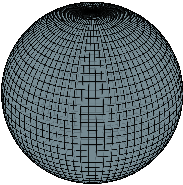
\includegraphics[height=7em]{sphere_grid_equirectangular}
	\hfill
	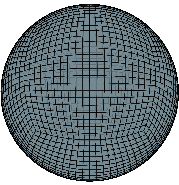
\includegraphics[height=7em]{sphere_grid_cubedsphere}
	\hfill
	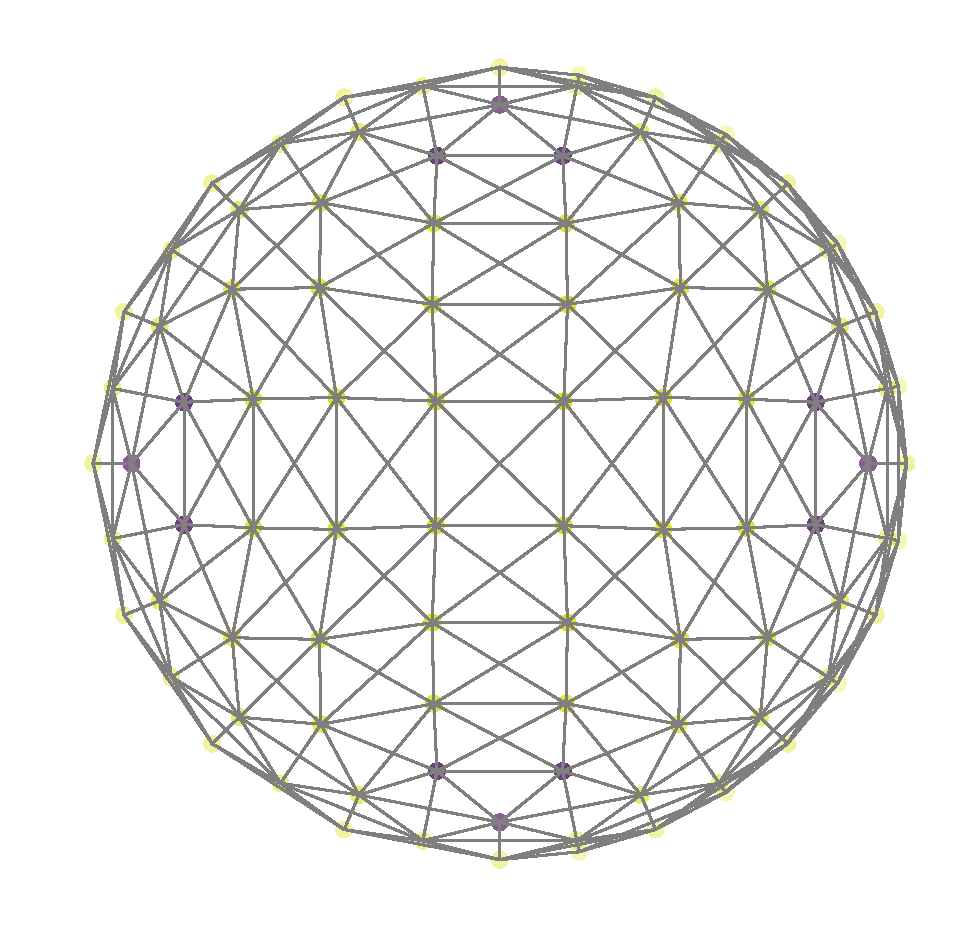
\includegraphics[height=7em]{half_graph_4}
	\caption[]{Some pixelizations of the sphere. Left: the equirectangular grid, using equiangular spacing in a standard spherical-polar coordinate system. Middle: an equiangular cubed-sphere grid, as described in \citet{ronchi1996cubed}. Right: graph built from an HEALPix pixelization of half the sphere ($N_{side} = 4$). By construction, each node has 8 neighbors, except the highlighted ones which have only 7.\footnotemark[7] Left and middle figures are taken from \citet{boomsma2017spherical}.}
	\label{fig:sphere_grids}
	\label{fig:healpix_graph_4}
\end{figure}

% As presented by~\cite{cohen2018spherical}, the most mathematical approach to extend the convolution on a sphere is to use a spherical Fourier transform. The convolution is then simply defined as the product in the spectral domain. This approach requires one Fourier and one inverse Fourier transform per convolution which remain, even with accelerated algorithms, expensive.

\citet{cohen2018spherical} leverages the continuous spherical convolution. The goal of this contribution was to define a rotation-equivariant convolution on the sphere, i.e., a rotation of the input implies the same rotation in the output.
The resulting convolution is performed by (i) a spherical harmonic transform (SHT), i.e., a projection on the spherical harmonics, (ii) a  multiplication in the spectral domain, and (iii) an inverse SHT. Hence the computational cost of a convolution is essentially due to the two SHTs. A naive implementation of the SHT costs $\bO(N_{pix}^2)$ operations, where $N_{pix}$ is the number of pixels. There fortunately exists accelerated schemes for some sampling sets, see for example \citet{mohlenkamp1999fast, rokhlin2006fast, reinecke2013libsharp}.
The main advantage of this approach is that it provides a mathematically well defined rotation-equivariant network. Nevertheless, even with accelerated SHTs, the convolutions remain expensive, limiting the practical use of this approach.
For example with the HEALPix sampling, which was designed to have a fast SHT by being iso-latitude, the computational cost of the SHT is $\bO(N_{pix}^{3/2}) = \bO(N_{side}^3) = \bO(\ell_{max}^3)$, where $\ell_{max}$ is the largest order (angular frequency) \citep{gorski2005healpix, reinecke2013libsharp}.\footnote{All pixels are placed on $N_{ring} = 4N_{side}-1 = \bO(\sqrt{N_{pix}})$ rings of constant latitude. Each ring has $\bO(\sqrt{N_{pix}})$ pixels. Thanks to this iso-latitude property, the SHT is computed using recurrence relations for Legendre polynomials on co-latitude and fast Fourier transforms (FFTs) on longitude. The computational cost is thus $\sqrt{N_{pix}}$ FFTs for a total cost of $\bO(N_{pix} \log(\sqrt{N_{pix}}))$, plus $\sqrt{N_{pix}}$ matrix multiplications of size $\sqrt{N_{pix}}$ for a total cost of $\bO(N_{pix}^{3/2})$.}
In comparison, filtering with our method scales as $\bO(N_{pix})$ (see \secref{efficient_convolution}). Moreover, \figref{filtering_speed} shows that a naive implementation of our method is more than ten times faster than the SHT implemented by the highly optimized \pkg{libsharp} library used by HEALPix \citep{reinecke2013libsharp}.
While a comparison is theoretically possible, the experiments of~\cite{cohen2018spherical} are done using the geodesic grid sampling set and do not provide any code for the HEALPix one. Hence, a practical comparison is not possible.
We also note that this approach cannot be easily accelerated when data lies on a part of the sphere only. That is an important use case in cosmology as measurements are often partial, i.e., full-sky maps are rare. One could still fill the unseen part of the sphere with zeros, and avoid to compute empty integrals (on the latitude or longitude). It is however not straightforward to identify those empty directions, and computations would still be wasted (consider for example a ring which mostly contains zeros but a few measurements). With graphs however, one only pays for the used pixels. The cost is some distortions due to border effects (see \figref{border_effects} and \ref{sec:border_effects}). Those can however be mitigated by padding with zeros a small area around the measurements.


A second direction has been followed in~\citet{boomsma2017spherical}. The idea is
to use the traditional 2-dimensional convolution on an irregular grid defined on the
sphere. In the paper, two grids are used: the equirectangular grid, and the cubed-sphere grid defined by~\citet{ronchi1996cubed}. See \figref{sphere_grids}. Because this
approach is based on the classic 2-dimensional convolution, it benefits from all the optimizations developed for images and is very likely to be
the most computationally efficient one. However, it suffers that it can only be used using very
specific grid sampling sets which are not including HEALPix. Furthermore, the
grid requirement makes it impossible for the convolution to capture the
spherical properties of the domain, i.e., the cubed-sphere sampling is by
definition adapted to a cube and not to a sphere.
Those samplings are not ideal as their resolution is not constant across the sphere. Indeed, the singularities --- the poles for the equirectangular grid, the corners of the cube for the cubed-sphere --- are over-sampled. Equal areas of discrete elements is advantageous for physical measurements as white noise at the sampling frequency of the instrument gets integrated exactly into white noise in the pixel space, and sky signals are sampled without regional dependence.
% \nati{Michael: Under some very specific hypothesis, this second approach is a particular case of our method, i.e. (i) our method with a stupid sampling, (ii) assumption that graph convolution on a grid == 2d convolution. Do you think we should mention that? I think we should not.}

In an attempt to get the best of the first two approaches, we follow a third
direction. We use a graph to adapt to the particular structure of the sphere.
While the convolution remains efficient, it still captures well the spherical
structure and is particularly adapted to the HEALPix sampling.

The use of a graph to model the discretized sphere was considered by~\citet{khasanova2017graphomni} as well. The authors map omnidirectional images to the sphere, with the goal of correcting for distortions induced by the lens used for the acquisition.
Besides the different application covered by the paper, there are two important
differences. First the sampling is different as~\cite{khasanova2017graphomni} uses a
grid. Second, it uses a different graph CNN based on a different parameterization
of the convolution kernel.
As~\citep{boomsma2017spherical}, they use an equirectangular grid sampling. Moreover, they did not take advantage of a hierarchical pixelization of the sphere and resorted to dynamic pooling~\citep{kalchbrenner2014dcnn}.
Finally, while we do want our network to be rotation invariant, their statistical layer --- an operation which computes a set of spatially invariant statistics of the last feature map --- destroys a lot of information \todo{and hinders performance (should be empirically verified)}. Moreover, the chosen statistics have to be hand-crafted to capture statistics of interest. While developing completely invariant transforms is a  goal worth investigating, CNNs for image recognition (arguably the most researched and developed architectures), are not built to be fully invariant to translation. As with the proposed spherical CNN, the fully connected layers at the end of the network depend on the spatial localization of features. While that may not be ideal, it was shown to work well in practice.
\todo{In this work we reused the idea of a statistical layer, described in \secref{stat_layer}, to provide invariance to isometric transformations such as translation and rotation on the sphere. While \citet{khasanova2017graphomni} uses the mean and variance of diffused versions of the last feature maps, we experimentally tested multiple variants and got good results by keeping all the statistical moments via a learned histogram. That is similar to the learnable histogram introduced by \citet{wang2016learnhist}, although for the orthogonal purpose of integrating global context in object detection and segmentation tasks.}

There exists many formulations of graph neural networks, reviewed by \citet{bronstein2017review} and \citet{hamilton2017review}. For this contribution, we chose the formulation of \citet{defferrard2016convolutional} as its root on strong graph signal processing theory makes the concept of convolutions and filters explicit \citep{shuman2013emerging}. Its tie to a graph Fourier transform allows us to compare with the spherical harmonic transform, and study its invariance properties. More geometric than permutation invariant aggregation. A contrario, formulations with exploit the tengant space of manifolds define a local coordinate system. While this formulation of convolution can learn anisotropic filters, it is not equivariant to translation. \todo{better wording}
\todo{three main interpretations: gsp, Bronstein manifold tangent plane, message passing, permutation invariant aggregation, spatial formulations}
Bronstein is a spatial formulation where the registration is done by projection on the tangent plane.
% Not Bronstein's manifold approach as we want a Fourier basis to compare to the spherical harmonics.
% Be as close as possible to spherical harmonics.
Related to this, convolutional neural networks have been defined on manifolds and have achieved impressive results on shapes [Bronstein]. They however too depend on an orientation, which spheres do not possess.

% Anisotropic cannot be invariant

The connection has recently been made between graph CNNs and group equivariant CNNs \cite{kondor2018equivariance}, justifying the use of graphs to gain rotation equivariance on the sphere.

In this work, we are using the graph CNN formulation introduced in~\cite{defferrard2016convolutional}.

Spatial definitions of graph convolutions, e.g. [Niepert] needs to define an orientation in order to match the edges with the filters. Most often the orientation is not given by the application, and one has to define it (for example by ordering by degree or any other measure, or by using a graph coloring). There is no good default good orientation on general graphs and the choice of an orientation is highly application dependent.

\section{Method}
\label{sec:method}
% \begin{itemize}
% 	\item We build a graph using the healpix sampling
% 	\item Define Fourier transform and show that the harmonics are visually close to the spherical harmonics
% 	\item Define spherical convolution using the graph Fourier transform and show heat diffusion example
% 	\item Show the limits of the approach and explain why we cannot have a perfect spherical convolution with this technique
% \end{itemize}

A CNN is composed of the following main building blocks~\citep{lecun1998cnn}: (i) a convolution, (ii) a non-linearity, (iii) a down-sampling operation, (iv) a pooling operation, and (v), optionally, some normalization.\footnote{\citet{ioffe2015batchnorm} have shown that batch normalization helps training. We verified this experimentally in our setting as well.} Our architecture is depicted in~\figref{architecture} and discussed in greater details in \secref{architecture}. As operations (ii) and (v) are point-wise, they do not depend on the data domain. The pooling operation is simply a permutation invariant aggregation function which does not need to be adapted either. The convolution and down-sampling operations however need to be generalized from Euclidean domains to the sphere.

On regular Euclidean domains, such as 1-dimensional time series or 2-dimensional images, a convolution can be efficiently implemented by sliding a localized convolution kernel (for example a patch of 5x5 pixels) in the signal domain. Likewise, down-sampling can be achieved by taking one pixel out of $n$.
Because of the irregular sampling, there is no straightforward way to define a convolution on the sphere directly in the pixel domain.

We will hence make a detour by the spectrum to perform the convolution.\footnote{Note that we only use the spectrum to define the convolution. The implementation however does not need a direct access to the spectrum, which is computationally much more efficient. See \secref{efficient_convolution}.}
The gist of our method is to define the convolution on a sphere using a graph, and the down-sampling using a hierarchical pixelization of the sphere.

\subsection{HEALPix sampling}
\label{sec:healpix}

Before doing any numerical analysis on the sphere, one first has to choose a tessellation, i.e., an exhaustive partition of the sphere into finite area elements, where the data under study is quantized.
The simplicity of the spherical form belies the intricacy of global analysis on the sphere. There is no known point set which achieves the analogue of uniform sampling in Euclidean space and allows exact and invertible discrete spherical harmonic decompositions of arbitrary but band-limited functions. Any existing proposition of practical schemes for the discrete treatment of such functions on the sphere introduces some systematic error dependent on the global properties of the point set.
While our method is applicable to any pixelization of the sphere, two details depend on the chosen sampling: (i) the choice of neighbors in the construction of the graph, and (ii) the choice of parent nodes when coarsening the graph.
As HEALPix~\citep{gorski2005healpix} is the most popular sampling used in cosmology, our target application, we'll tailor the method to that particular sampling in the subsequent exposition.
%We'll note in later sections where the method should be adapted for a different sampling.

HEALPix is a particular case of a more general class of schemes which are based on a hierarchical subdivision of a base polyhedron.
%Many discretized maps of the sphere are based on a hierarchical subdivision of a base polyhedron.
Another example is the geodesic grids which are based on geodesic polyhedrons, i.e., polyhedrons made of triangular faces. A counter-example is the equirectangular projection, which is not constructed from a base polyhedron, although it can be subdivided.
In the particular HEALPix case, the base is a rhombic dodecahedron, i.e., a polyhedron made from 12 congruent rhombic faces.\footnote{A rhombus is a quadrilateral whose four sides all have the same length.} See \figref{pooling} for an illustration of the base rhombic dodecahedron and its subdivisions.

HEALPix is an acronym for Hierarchical Equal Area isoLatitude Pixelization of a sphere. As suggested in the name, this pixelization produces a hierarchical subdivision of a spherical surface in which each pixel covers the same surface area as every other pixel.
A hierarchy is desired for data locality in computer memory. Equal area is advantageous because white noise generated by the signal receiver gets integrated exactly into white noise in the pixel space. Isolatitude is essential for the implementation of a fast spherical transform. HEALPix is the sole pixelization scheme which satisfies those three properties.

The lowest possible resolution is given by the base partitioning of the surface into $N_{pix} = 12$ equal sized pixels (right-most sphere in \figref{pooling}). As each pixel is subdivided in four, the second coarser resolution is $N_{pix} = N_{side}^2 \cdot 12 = 2^2 \cdot 12 = 48$ pixels (middle sphere in \figref{pooling}), the third is $N_{pix} = N_{side}^2 \cdot 12 = 4^2 \cdot 12 = 192$ pixels, etc., where $N_{side} = 1, 2, 4, 8, \ldots$ is the grid resolution parameter.
High-resolutions HEALPix maps easily reach millions of pixels. \figref{example_maps} shows two examples.

\begin{figure}
	\centering
	\begin{subfigure}[b]{0.45\linewidth}
		\centering
		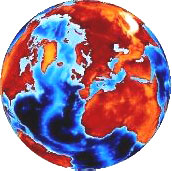
\includegraphics[width=\linewidth]{exampleEarthTopo}
		\caption{}
		\label{fig:example_earth}
	\end{subfigure}
	\hfill
	\begin{subfigure}[b]{0.45\linewidth}
		\centering
		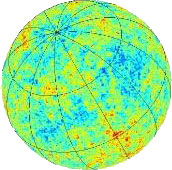
\includegraphics[width=\linewidth]{exampleCMB}
		\caption{}
		\label{fig:example_cmb}
	\end{subfigure}
	\caption[]{Example of (a) an Earth topography map composed of \textasciitilde 3 million pixels (\textasciitilde 7 arcmin resolution) and (b) a model of the Cosmic Microwave Background (CMB) radiation temperature anisotropy, composed of \textasciitilde 13 million pixels (\textasciitilde 3.4 arcmin resolution).\footnotemark}
	\label{fig:example_maps}
\end{figure}

\footnotetext{Figures from \url{https://healpix.jpl.nasa.gov/}.}

\subsection{Graph construction}

Our graph is constructed as an approximation of the continuous 2D manifold that is the surface of the sphere. Indeed, \citet{belkin2007convergence} showed that the graph Laplacian converges to the Laplace-Beltrami when the number of pixels goes to infinity. That construction can accommodate any sampling, regular or not.

From the HEALPix pixelization, we build a weighted undirected graph $\G = (\V, \E, \W)$, where $\V$ is the set of $N_{pix} = |\V|$ nodes, $\E$ is the set of edges, and $\W$ is the weighted adjacency matrix. In our graph, each pixel $i$ is represented by a node (also called vertex) $v_i \in \V$. Each node $v_i$ is then connected to the $8$ (or $7$)\footnote{\label{neighbors}The $12 \cdot 4 = 48$ pixels at the corner of each rhombus of the base dodecahedron only have 7 neighboring pixels. See Figures~\ref{fig:healpix_graph_4} and~\ref{fig:pooling}.} nodes $v_j$ which represent the neighboring pixels $j$ of pixel $i$, forming edges $(v_i, v_j) \in \E$. Given those edges, we define the weighted adjacency matrix $\W \in \R^{N_{pix} \times N_{pix}}$ as
\begin{equation*}
	\W_{ij} = \begin{cases}
		\exp \left( -\frac{\|\x_i-\x_j\|_2^2}{\sigma^2} \right) & \text{if pixels $i$ and $j$ are neighbors,} \\
		0 & \text{otherwise,} \\
	\end{cases}
\end{equation*}
where $\x_i$ is a vector encoding the 3-dimensional coordinates of pixel $i$, and
\begin{equation*}
	\sigma = \frac{1}{|\E|} \sum_{(v_i, v_j) \in \E} \|\x_i-\x_j\|_2
\end{equation*}
is the average Euclidean distance over all connected pixels. This weighting scheme is important as while pixel areas are equal, distances between pixels are not.
Other weighting schemes are possible. For example,~\cite{khasanova2017graphomni} uses the inverse of the distance instead. We found out that the one proposed above works fine for our purpose.
\figref{healpix_graph_4} shows a graph constructed from the HEALPix sampling of a sphere.

% mdeff: Why not $1/d$? See Pascal's paper
% nati: The question is: is $1/d$ also good when we have 7/8 neighbors instead of 4? Practically, we can also use $1/d$, but that means changing the code and re-runing the experiment. We probably do not have to change any parameter though... @mdeff: do you think we should try this for this paper? Or we keep that for the next one.
% mdeff: I tried and the eigenvectors and eigenvalues are mostly the same. To me, there is no point in trying for trying. We should rather come up with a definition of distance that will make the eigenvectors closer to the real spherical harmonics.
% Agreed: I added a reference to Pascal paper.

\subsection{Graph Fourier basis}

Following~\cite{shuman2013emerging}, the normalized graph Laplacian,
defined as $\L = \I - \D^{-1/2} \W \D^{-1/2}$, is a second order differential operator
that can be used to define a Fourier basis on the graph. Here $\D$ is the diagonal
matrix where $\D_{ii} = \b{d}_i$ and $\b{d}_i = \sum_j \W_{ij}$ is the weighted degree of node $v_i$. By construction, the Laplacian is symmetric positive
semi-definite and hence can be decomposed as $\L = \U \bLambda \U\trans$, where $\U = [\b u_1, \ldots, \b u_{N_{pix}}]$ is an
orthonormal matrix of eigenvectors and $\bLambda$ is a diagonal matrix of
eigenvalues. The graph Fourier basis is defined as the Laplacian eigenvectors, motivated by the fact that a Fourier basis should diagonalize the Laplacian operator.
The graph Fourier transform of a signal $\f \in \R^{N_{pix}}$ is simply its projection on the eigenvectors given by
$\hat{\f} = \mathcal{F}_\G \{\f\} = \U\trans \f$. It follows that the inverse graph Fourier transform reads $\mathcal{F}^{-1}_\G \{\hat{\f}\} = \U\hat{\f} = \U \U\trans \f = \f$.
Note that the Fourier modes are ordered in the increasing order of the Laplacian eigenvalues $\bLambda$, which can be interpreted as squared frequencies.
Indeed,
\begin{equation*}
	\bLambda_{ii} = \b u_i\trans \L \b u_i = \sum_{(v_j, v_k) \in \E} \frac{\W_{jk}}{\sqrt{\b d_j \b d_k}} (\U_{ji} - \U_{ki})^2
\end{equation*}
is a measure of the variation of the eigenvector $\b u_i$ is on the graph defined by the Laplacian $\L$.

\begin{figure}
	\centering
	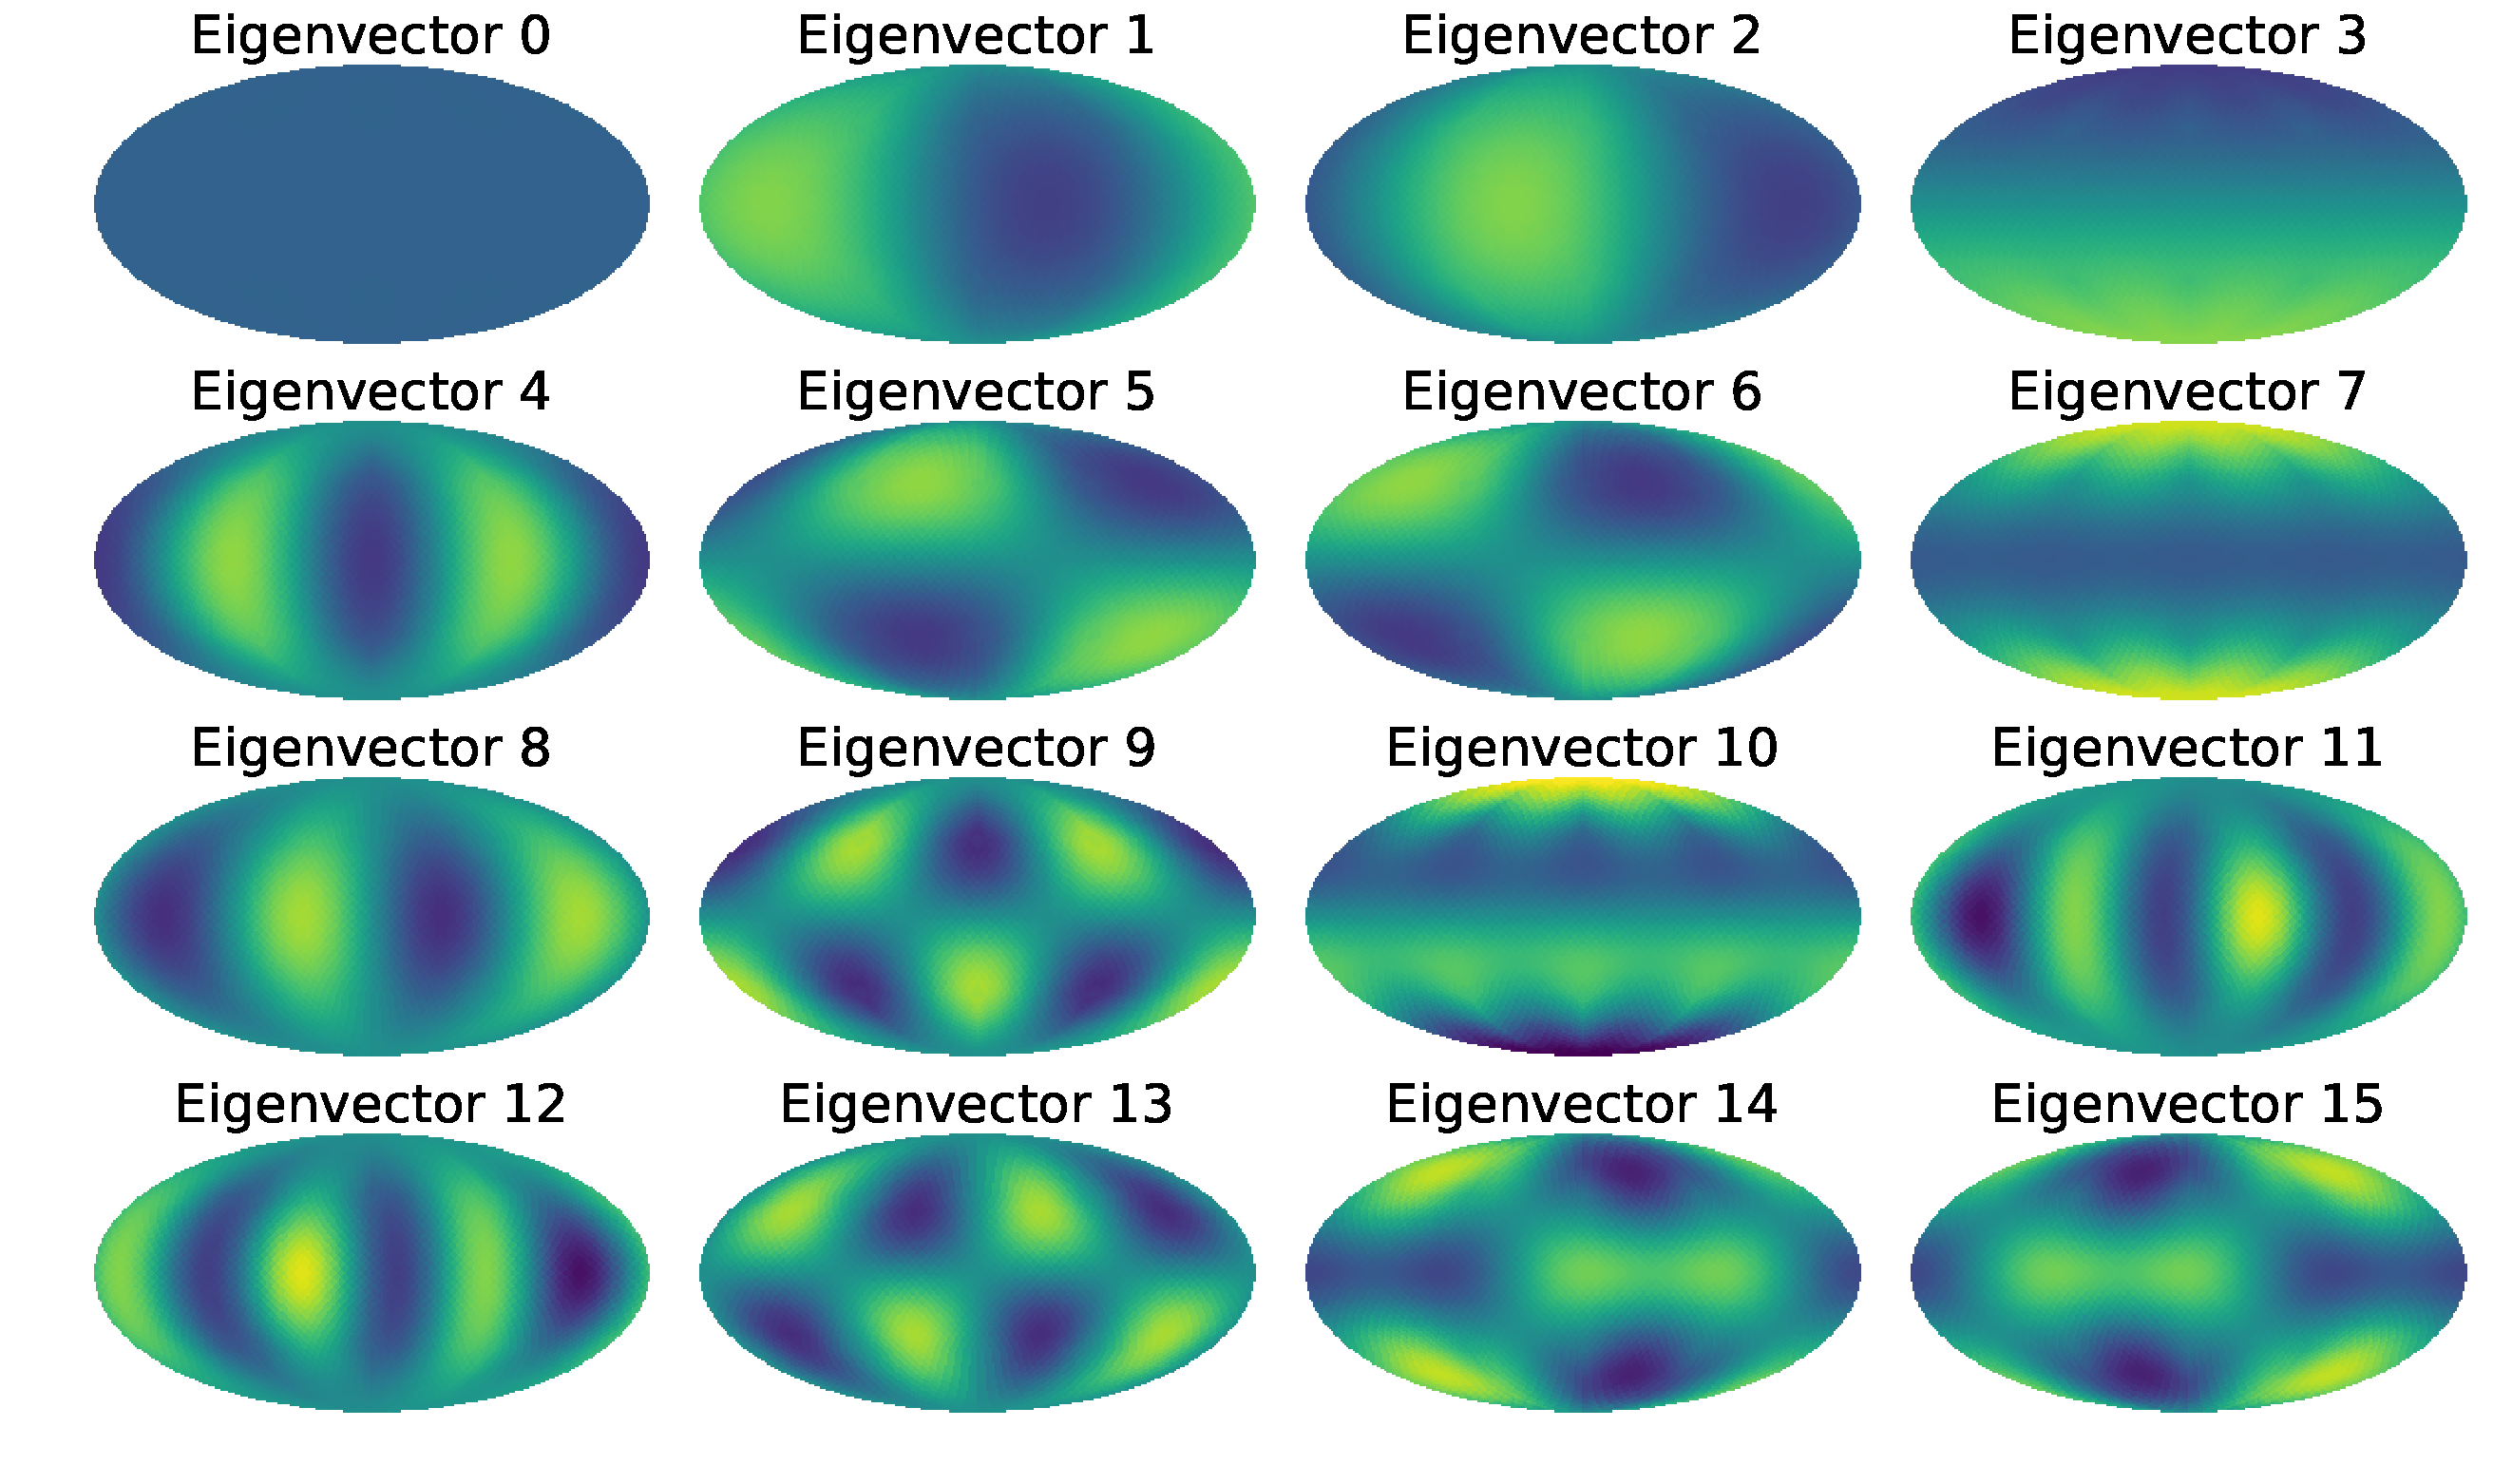
\includegraphics[width=\linewidth]{eigenvectors}
	\caption{The first 16 Fourier modes (eigenvectors of the graph Laplacian) of a graph constructed from the HEALPix sampling of the sphere. Eigenvectors 1--3 could be associated with spherical harmonics of degree $\ell=1$ and order $|m|=(0,1)$, eigenvectors 4--8 with degree $\ell=2$ and order $|m|=(0,1,2)$, and eigenvectors 9--15 with degree $\ell=3$ and order $|m|=(0,1,2,3)$. Nevertheless, the graph eigenvectors are \emph{only approximating} the real spherical harmonics.}
	\label{fig:graph_harmonics}
\end{figure}

It turns out that using the graph construction described above, the graph Fourier modes resemble the spherical harmonics (see \figref{graph_harmonics}). That is a strong hint that the graph is able to capture the spherical properties of the HEALPix sampling. This topic is further discussed in \ref{sec:comparison_spherical_harmonics}.

\subsection{Convolution on graphs}
\label{sec:graph_convolution}

As there is no notion of translation on a graph, we cannot really convolve two graph signals. We can, however, convolve a signal with a kernel defined in the spectral domain. More precisely, we are filtering a graph signal by a kernel. Given the convolution kernel
$h: \R_+ \rightarrow \R$, a signal $\f \in \R^{N_{pix}}$ on the graph is filtered as
\begin{equation} \label{eqn:graph_convolution}
	h(\L) \f = \U h(\bLambda) \U\trans \f,
\end{equation}
where $h(\bLambda)$ is a diagonal matrix where $h(\bLambda)_{ii} = h(\bLambda_{ii})$, and $h(\bLambda) \hat{\f}$ is the spectral representation of $\f$ after filtering.

Contrary to classical signal processing on Euclidean domains, the kernel $h$ has no single representation in the vertex domain and cannot be translated on the graph. It can however be localized on any vertex $v_i$ by the convolution with a Kronecker delta $\b \delta_i \in \R^{N_{pix}}$,\footnote{A Kronecker delta is the signal $\b \delta_i \in \R^{N_{pix}}$ that is zero everywhere except on vertex $v_i$ where it takes the value one.} that is $h(\L) \b \delta_i$, a column of $h(\L)$.
This localization can be useful to visualize kernels as explained in~\ref{sec:filter_visualization}.
If the graph is not regular, i.e., all nodes don't have the same number of neighbors, and all distances are not equal, the effect of the kernel will slightly differ from one node to another. While there is no perfect sampling of the sphere, these differences are negligible as the structure of the whole graph is very regular. However, when considering only parts of the sphere, one can observe important border effects (see \figref{border_effects} and~\ref{sec:border_effects}).
Finally, the graph convolution can be interpreted in the vertex domain as a scalar product with all localizations of the kernel:
\begin{equation} \label{eqn:graph_convolution_spatial}
	(h(\L) \f)_i = \langle h(\L) \b \delta_i, \f \rangle.
\end{equation}
\textbf{Example.}
Let us consider the heat diffusion problem
\begin{equation} \label{eqn:heat_equation}
	\L \b{f}(t) = \tau \partial_t \b{f}(t),
\end{equation}
where $\b{f}: \R_+ \rightarrow \R^{N_{pix}}$. Given the initial condition
$\b{f}(0)$, the solution of~\eqnref{heat_equation} can be expressed as
\begin{equation*}
	\b{f}(t) = e^{-\L \tau t} \b{f}(0) = \U e^{-\bLambda t \tau} \U\trans \g{f}(0) = K_t(\L) \b{f}(0),
\end{equation*}
which is, by definition, the convolution of the signal $\b{f}(0)$ with the kernel $K_t(\lambda)=e^{-\tau t \lambda}$. Since the kernel $K_t$ is applied to the graph eigenvalues $\bLambda$, which can be interpreted as squared frequencies, it can also be considered as a generalization of the Gaussian kernel on the sphere. \figref{gaussian_filters_comparizon} shows the effect of the convolution by diffusing a unit of heat for $\tau=1$ at various times $t$. By comparing the graph convolution with the spherical symmetric Gaussian smoothing, we observe that both techniques lead to similar results (see \figref{gaussian_filters_comparizon}). While the graph convolution remains different from the spherical convolution, this small experiment shows that, providing the correct parameters, graph convolution can approximate spherical convolution. For additional insides about the graph kernel $K_t$, we refer to the \figref{gaussian_filters_visualization} and~\ref{sec:filter_visualization}.

\begin{figure}
	\centering
	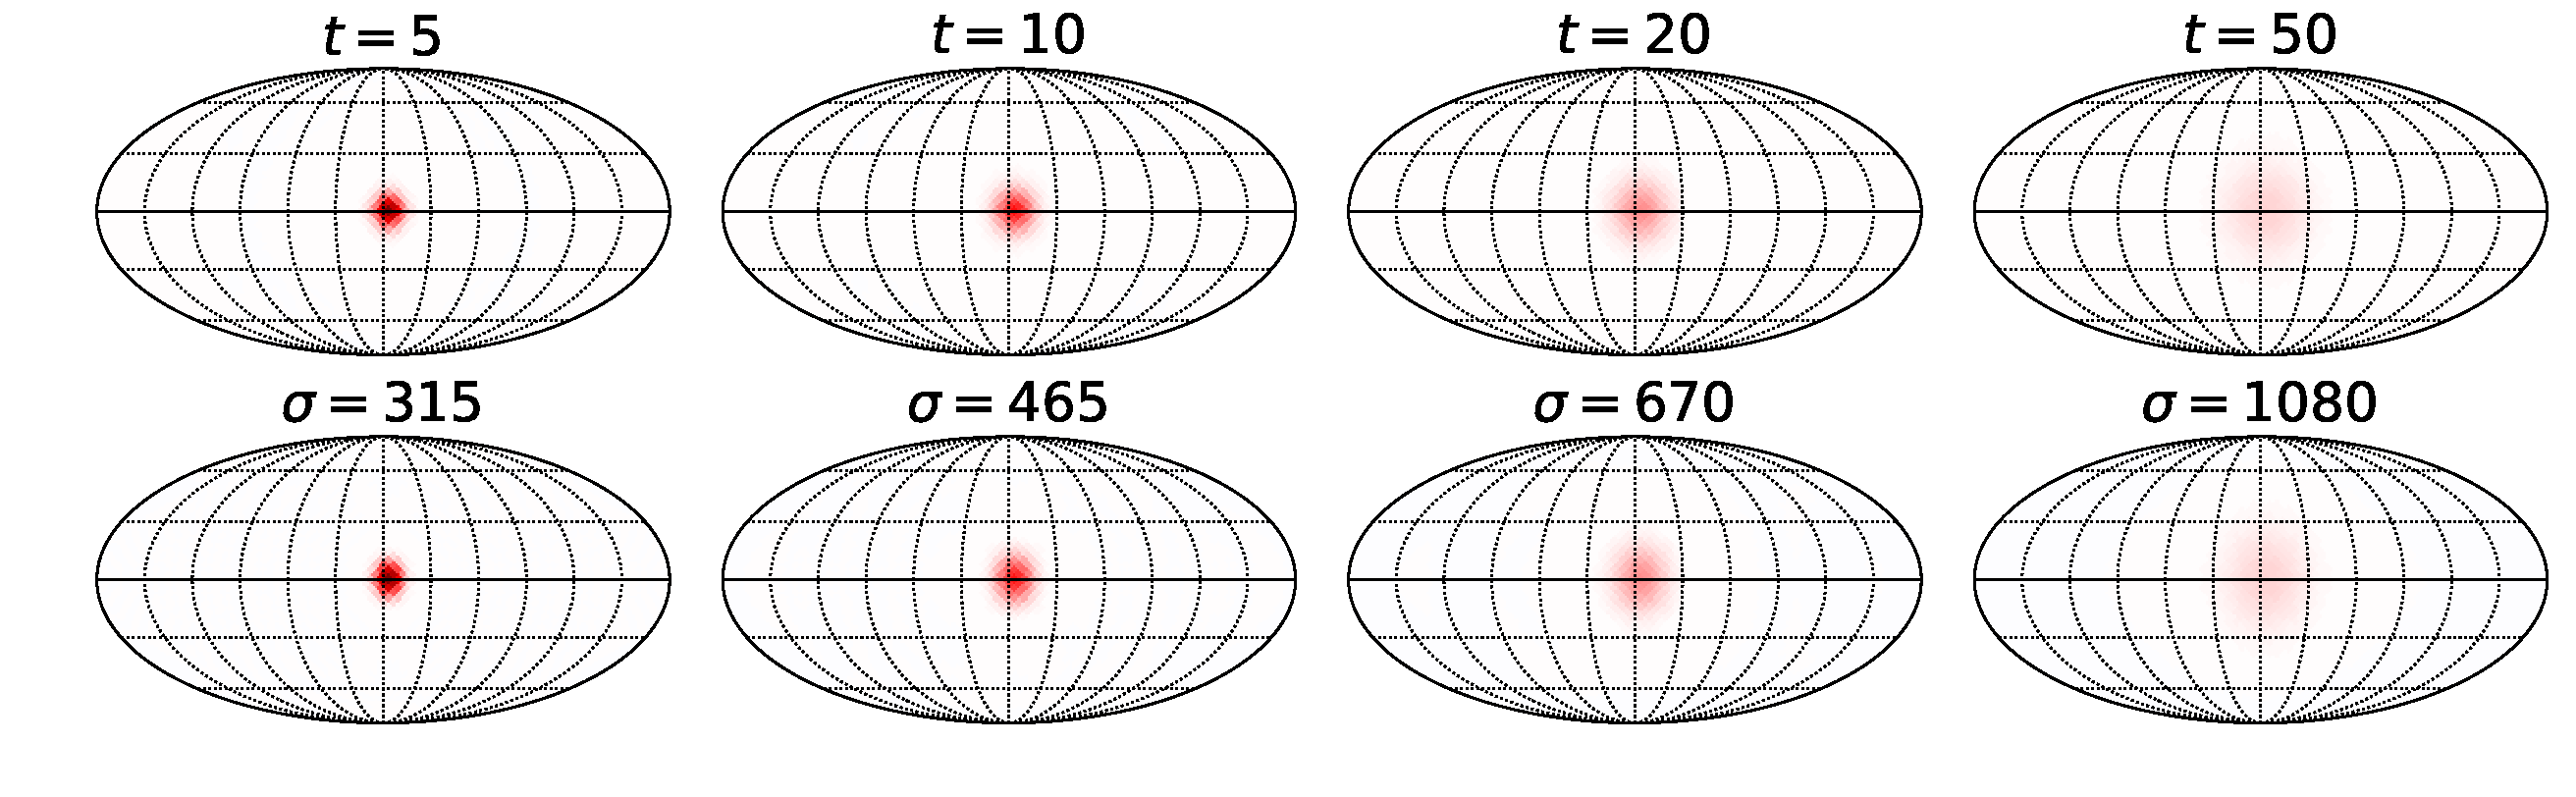
\includegraphics[width=\linewidth]{gaussian_filters_sphere}
	\caption{Comparison of convolution with the graph and the spherical harmonics ($N_{side} = 16$).
	Top: Diffusion of a unit of heat for different times $t$ using the graph.
	Bottom: spherical symmetric Gaussian smoothing for different $\sigma$ (arcmin).
	Relative difference between graph convolution and spherical smoothing: $10.4$\%, $5.7$\%, $4.8$\%, $3.8$\%.
	\todo{(i) Only three diffusion steps to have a bigger figure? \nati{Agreed! Will do soon!}}
\todo{(ii) The main issue with our filters is that their shape depends on the localization. It would be nice to measure the expectation and variance of the error over all locations. That would show how severe the distortion is.}
\nati{Let us keep that for the next paper. I am quite sure, it is negligible in this particular case.}}
	\label{fig:gaussian_filters_comparizon}
\end{figure}

Furthermore, this result is another sign that the constructed graph is able to capture the spherical
structure of the HEALPix sampling. In some applications, where the
exactitude of the convolution is not a requirement, such as de-noising, graph convolution could be used instead of using the spherical harmonics.
The fact that both convolutions are not identical is not relevant in a neural network setting, as the convolution kernels are learned anyway.
% not ideal tho as the graph convolution depends on the localization

\subsection{Efficient convolutions}
\label{sec:efficient_convolution}

While \eqnref{graph_convolution} is a theoretically well justified definition of the convolution of a graph signal $\f$ by a kernel $h$, it is computationally cumbersome. As there exists no general fast Fourier transform (FFT) for graphs,\footnote{See \citep{le2018fgft} for a comparison between the polynomial definition of filters presented here and a class of fast graph Fourier transforms based on the approximation of the Fourier basis $\U$ by a product of sparse matrices.} the Fourier transform, i.e., the multiplication of the signal $\f$ by the dense matrix $\U$, costs $\bO(N_{pix}^2)$ operations. In a CNN, this operation has to be performed for each training step (forward and backward). As current training procedures are not data efficient and require a lot of samples, a quadratic computational cost in the sample size is a show stopper.
Moreover, the eigendecomposition of the Laplacian $\L$ is needed to obtain the Fourier basis $\U$ in the first place. That has a unique cost of $\bO(N_{pix}^3)$ operations.

Forunately, both of these computational issues can be overcome by defining the convolution kernel $h$ as a polynomial $h_\theta(\lambda) = \sum_{k=0}^K \theta_k \lambda^k$ of degree $K$ parameterized by $K+1$ coefficients $\theta$. In that specific case, the filtering operation \eqnref{graph_convolution} becomes
\begin{equation} \label{eqn:graph_convolution_polynomial}
	h_\theta(\L) \f =  \U \left(\sum_{k=0}^K \theta_k \bLambda^k \right) \U\trans \f = \sum_{k=0}^K \theta_k \L^k \f,
\end{equation}
an operation requiring $k$ multiplication of the graph Laplacian matrix $\L$.
In our case, the Laplacian is extremly sparse ($8-9$ entries per line), making the filtering operation for a fixed $K$ linear in the number of pixel $N_{pix}$.
Moreover, here happens the transition from filtering in the spectral domain to filtering in the vertex domain. The matrix $\L^k$ captures $k$-neighborhoods of each pixel, i.e., $(\L^k)_{ij}$ is non-zero if and only if nodes $v_i$ and $v_j$ are connected by a path of length $k$.
As such, filtering with a polynomial convolution kernel can be interpreted in the pixel (vertex) domain as a weighted linear combination of the pixels neighbors values. The weights are determined by the filter coefficients $\theta$ and the Laplacian $\L$.
We note that restricting the graph convolutional kernel to a polynomial is similar to restricting the classical Euclidean signal-domain convolution to a patch. In the classical setting, the convolution with a patch is simply a weighted sum of the neighbors with the weights defined by the patch. Similarly, each lines of the matrix $\sum_{k=0}^K \theta_k \L^k$ defines an "irregular patch of radius $K$" for our irregular domain.
\todo{Better vertex domain explanation. \nati{I gave it a try. Should we take a single vertex and explain what heppens to it? Note that I suppressed the following paragraph. }}

% To make the parallel with classical Euclidean signal-domain convolution, i.e., filtering by multiplying the signal with translated versions of a patch, we here match our filter at the level of neighborhoods\footnote{The 1-neighborhood of a node is the set of nodes which are directly connected to it. The 2-neighborhood is the set of nodes which are connected through paths of length 2.} rather than individual nodes. That is required as there is no notion of ordering in a general graph. For example, in a classical convolution on the grid, the relative ordering of vertices is up, down, left, and right. There is no such ordering on the sphere either, especially if irregularly sampled.

Following \citet{defferrard2016convolutional}, we define our filters as Chebyshev polynomials such as the convolution operation becomes
\begin{equation} \label{eqn:graph_convolution_cheby}
	h_\theta\left(\tL\right) \f = \U \left(\sum_{k=0}^K \theta_k T_k\left(\tilde{\bLambda}\right) \right) \U\trans \f = \sum_{k=0}^K \theta_k T_k\left(\tL\right) \f,
\end{equation}
where $\tL = \frac{2}{\lambda_{max}} \L - \b{I} = -\frac{2}{\lambda_{max}} \D^{-1/2} \W \D^{-1/2}$ is the rescaled Laplacian with eigenvalues $\tilde{\b \Lambda}$ in $[-1, 1]$ and $T_k(\cdot)$ is the Chebyshev polynomial of degree $k$, defined by the recursive relation $T_k(\tL) = 2\tL T_{k-1}(\tL) - T_{k-2}(\tL)$, $T_1(\tL) = \tL$, $T_0(\tL) = \b{I}$. While definitions \eqnref{graph_convolution_polynomial} and \eqnref{graph_convolution_cheby} both allow the representation of the same set of filters, Chebyshev polynomials are preferred as they form an orthogonal basis on the interval $[-1, 1]$. Moreover, they factor out $\tL^{k-2}$ from $T_k(\tL)$, e.g., the 3-neighborhood is not mixed with the 5-neighborhood. That results in easier learning when optimizing the parameters $\theta$.
Finally, the coefficients can be computed such as the truncated Chebyshev expansions gives an approximate minimax polynomial of a given filter \citep{hammond2011wavelets}. While that is irrelevant when learning filters, it is useful when smoothing a signal on the sphere by filtering it with an approximated low-pass filter.
In practice, we found out that Chebyshev polynomials are slightly more stable in our experiment. We believe that this is due to their orthogonality (as explained above) and uniformity\footnote{The amplitude of Chebyshev polynomials is more or less constant over the domain $[-1, 1]$ independently of the order $k$. On the contrary the amplitude of $x^k$ is very different for $|x|\approx 0$ and $|x| \approx 1$.}.
\nati{I added a sentence and I think we should not give much more details here. If we do an experiment, we can comment in the experiment section.}
\todo{(i) scale of $\theta_k$: they are mostly uniform for Chebyshev polynomials, end exploding for monomials. Though SGD implicitly imposes a uniform prior on the learned parameters.}
\todo{(ii) numerical stability of $\L^k \f$ v.s. $T_k(\L) \f$}
\todo{(iii) in the code, initialize $\theta_k$ with stdev adapted to $F_{in}$ and $K$}

Exploiting the recursive formulation of Chebyshev polynomials, evaluating \eqnref{graph_convolution_cheby} requires $\bO(K)$ multiplications of the dense vector $\f$ with the sparse matrix $\tL$. The cost of one such multiplication is $\bO(|\E|)$. By construction of our graph, $|\E| < 8 N_{pix}$. The overall computational cost of the convolution is thus reduced to $\bO(N_{pix})$ operations.
That is much more efficient than filtering with spherical harmonics, even tho the HEALPix sampling was designed to leverage a fast spherical transform (by being iso-latitude). That is especially true for smooth kernels which require a low polynomial degree $K$. See \figref{filtering_speed} for a speed comparison of low-pass filtering for Gaussian smoothing using the spherical harmonics and the presented method. It is ten to twenty times faster for $N_{side} = 2048$, with $K=20$ and $K=5$, respectively.

\begin{figure}
	\centering
	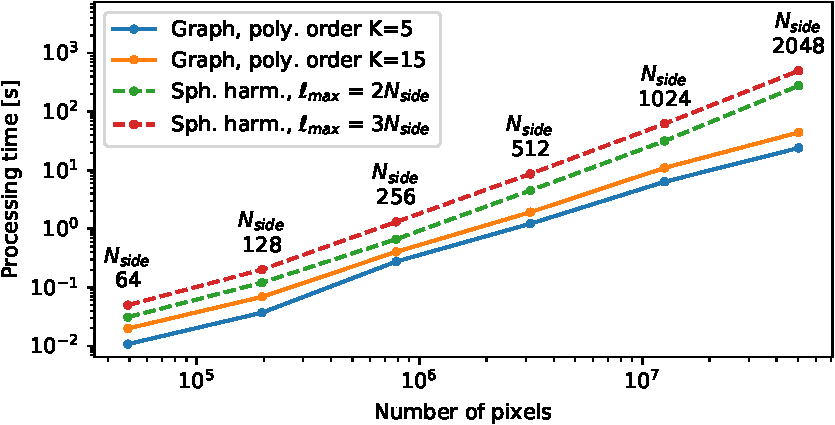
\includegraphics[width=\linewidth]{filtering_speed}
	\caption{Comparison of filtering speed for Gaussian smoothing of maps of various sizes. The fast spherical harmonic transform (SHT) is implemented by the healpy Python package (via the \texttt{healpy.sphtfunc.smoothing} function with $\ell_{max} = 3 N_{side} - 1$, the default.). The graph filtering is defined by \eqnref{graph_convolution_cheby} and implemented with the numpy and scipy Python packages. Both are executed on a single core. The theoretical cost of filtering on the graph is $\bO(K N_{pix})$ and $\bO(\ell_{max}^3)$ for the spherical harmonics, where $\ell_{max}$ is the largest degree (i.e., the spectrum is truncated at $\ell_{max}$).}
	\label{fig:filtering_speed}
\end{figure}

\subsection{Coarsening and Pooling}

Hierarchical pixelization schemes present a natural coarsening. Indeed, each subdivision divides a cell in an equal number of child sub-cells. Coarsening is the reverse operation: merging the sub-cells toward the goal of summarizing the data supported on them. Merging cells lead to a coarser graph, hence the name coarsening. Coarsening defines $\C(i)$, the set of children of node $v_i$. For the HEALPix subdivision scheme, the number of children is constant, i.e., $| \C(i) | = 4^p \ \forall i$, for some $p$.

Pooling refers to the operation that summarizes the data supported on the merged sub-cells in one parent cell. Given a map $\x \in \R^{N_{pix}}$, pooling defines $\y \in \R^{N'_{pix}}$ such as
\begin{equation} \label{eqn:pooling}
	y_i = f \left( \left\{ x_j : j \in \C(i) \right\} \right), \ \forall i \in [N'_{pix}],
\end{equation}
where $f$ is a function which operates on sets (possibly of varying sizes) and $N_{pix} / {N_{pix}}'$ is the down-sampling factor\footnote{$| \C(i) | = N_{pix} / {N_{pix}}' = (N_{side} / N'_{side})^2 = 4^p$ for HEALPix.}. That operation is often taken to be the maximum value, but it might be any permutation invariant operation such as the sum or the average. \figref{pooling} illustrates the process.

% The advantage of schemes based on a base polyhedron is that cells are equal-area. While that is not required for the convolution operation when modeling with graphs (it can be corrected by setting edge weights appropriately, see \citet{khasanova2017graphomni})
% nope: can also do a regular pooling on the equirectangular. It preserves the sampling, and the convolution is adapted to the sampling thanks to the edge weights.

\begin{figure}
	\centering
	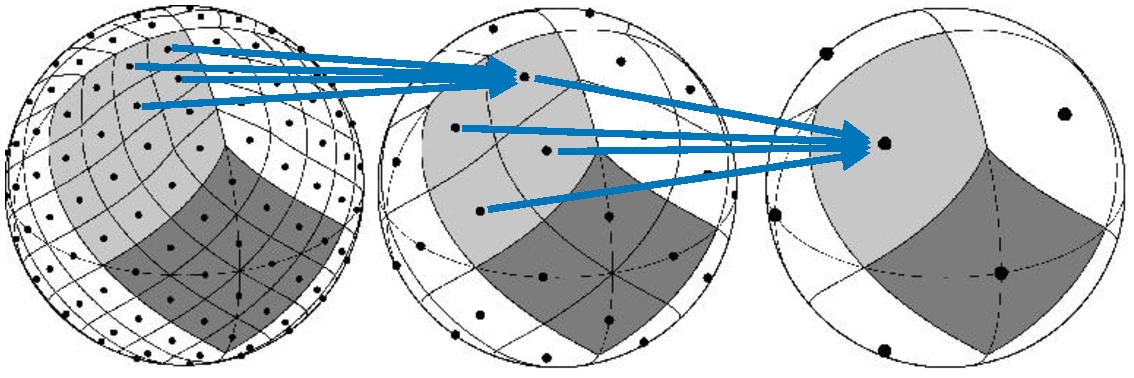
\includegraphics[width=\linewidth]{pooling}
	\caption{Two levels of coarsening and pooling: groups of 4 cells are merged into one, then the data on them is summarized in one. The coarsest cell covers $1/12$ of the sphere.}
	\label{fig:pooling}
\end{figure}

\subsection{Statistical layer}
\label{sec:stat_layer}
% Or Global pooling?

Following \citet{khasanova2017tigranet}, we use a statistical layer between the last graph convolutional layer and the first fully connected layer for the neural network to be invariant to isometric transformations such as rotation and translation of maps on the sphere. The role of the layer is to compute global and location independent statistics from feature maps. Besides providing invariance, the layer drastically compresses the representation of the data as the number of computed statistics $N_{stat}$ is usually much smaller than the size of the map, $N_{pix}$. That compression results in much smaller fully connected layers, the most parameter-hungry layers of a neural network. The invariance and reduced representation should help the network to learn from less samples and to generalize better to unseen data. Yet another advantage is that a network built with such a statistical layer is agnostic to the size of the input data, i.e., it can classify maps which do not have the same number of pixels. Indeed, such global summarization is invariant to node permutation and is commonly used along graph convolutions to classify graphs of varying sizes \citep{duvenaud2015gcn, li2015gatedgnn}.

Given a feature map $\x \in \R^{N_{pix}}$, the statistical layer is defined as
\begin{equation} \label{eqn:stat_layer}
	\y = f(\x) \in \R^{N_{stat}},
\end{equation}
where $f$ computes $N_{stat}$ statistics which are independent from the size of the map, $N_{pix}$. An example is the global average pooling $f(\x) = \esp(\x)$, introduced by \citet{lin2013globalavgpooling}, where $\esp(\x) = \frac{1}{N_{pix}} \sum_{i=1}^{N_{pix}} x_i$ is the empirical mean. Another example is $f(\x) = [\esp(\x), \var(\x)]\trans$, where $\var(\x) = \frac{1}{N_{pix}} \sum_{i=1}^{N_{pix}} (x_i - \esp(\x))^2$ is the empirical variance.

\todo{learned histogram \citep{wang2016learnhist} if it shows good results}

\todo{stats of diffused maps \citep{khasanova2017tigranet}. Provides stats at multiple scales?}

\todo{perf w.r.t. different functions $f$. Here or in the experiment section?}

\subsection{Graph convolutional neural network}
\label{sec:architecture}

Neural networks are constructed as stacks of layers which sequentially transform the data from its raw representation to a decision on the class label. Our architecture, pictured in \figref{architecture}, is composed of many layers. The convolutional part, the head of the neural network, is composed of graph convolutional layers (GC), pooling layers (P), and batch normalization layers (BN). The tail is composed of multiple fully connected layers (FC) followed by a softmax layer (SM). A statistical layer (ST) is optionally inserted between the convolutional head and the fully connected tail.

% As such, we will not mention the non-linearity in the description of our architectures.
A non-linear function $\sigma(\cdot)$ is applied after every linear GC and FC layer, except for the last FC layer where it is set to the identity. That operation is point-wise, i.e., $y_{ij} = \sigma(x_{ij})$ and $y_i = \sigma(x_i)$ for matrices $\X, \Y$ and vectors $\x, \y$. The rectified linear unit (ReLU) $\sigma(\cdot) = \max(\cdot, 0)$ is a common choice.

Given a matrix $\X = [\x_1, \ldots, \x_{F_{in}}] \in \R^{N_{pix} \times F_{in}}$, a GC layer computes $\Y = GC(\X) = [\y_1, \ldots, \y_{F_{out}}] \in \R^{N_{pix} \times F_{out}}$, where $N_{pix}$ is the number of pixels (and nodes), $F_{in}$ is the number of input features, and $F_{out}$ is the number of output features.
Using the efficient graph convolution from \eqnref{graph_convolution_cheby}, each output feature map is computed as
\begin{equation*}
	\y_i = \sum_{j=1}^{F_{in}} h_{\theta_{ij}}(\tL) \x_j + b_i \in \R^{N_{pix}}, \ \ \forall i \in [F_{out}].
\end{equation*}
As such, a GC layer is composed of $F_{in} \cdot F_{out}$ filters, each parameterized by $K$ numbers (see \secref{efficient_convolution}). A bias term $\b b \in \R^{F_{out}}$ is jointly optimized.
% only if batch normalization is not used

Given a matrix $\X \in \R^{N_{pix} \times F}$, a pooling layer computes $\Y = P(\X) \in \R^{N'_{pix} \times F}$ by reducing its spatial resolution ($N'_{pix} < N_{pix}$) according to \eqnref{pooling}.

Given a matrix $\X \in \R^{N_{pix} \times F}$, a batch normalization layer \citep{ioffe2015batchnorm} computes $\Y = BN(\X)$ such as
\begin{equation*}
	\y_i = \gamma_i \frac{\x_i - \esp(\x_i)}{\sqrt{\var(\x_i) + \epsilon}} + \beta_i, \ \forall i \in [F],
\end{equation*}
where $\gamma_{j}$ and $\beta_{j}$ are parameters to be learned and $\epsilon$ is a constant added for numerical stability. The empirical expectation $\esp(\x_i) \in \R$ and variance $\var(\x_i) \in \R$ are taken across training examples and pixels.
% the action of gamma can be done by the filters of the next layer

The statistical layer, defined in \eqnref{stat_layer}, independently transforms each of the $F$ feature maps of the input $\X \in \R^{N_{pix} \times F}$ into $\Y = ST(\X) \in \R^{N_{stat} \times F}$, where $N_{stat}$ is the number of statistics. One may even omit the FC layers and directly fed the output of the ST layer into the softmax layer, as proposed by \citet{lin2013globalavgpooling}. In this regime, $N_{stat} = 1$ and $F = N_{classes}$ is the number of classes to discriminate (i.e., the last GC layer outputs as many feature maps as there is classes).

A FC layer takes as input $\x \in \R^{F_{in}}$ and outputs
\begin{equation*}
	\y = FC(\x) = \b W \x + \b b \in \R^{F_{out}} ,
\end{equation*}
where $\W \in \R^{F_{out} \times F_{in}}$ and $\b b \in \R^{F_{out}}$ are the parameters to be learned.
Note that the output $\Y \in \R^{N_{pix} \times F_{out}}$ of the last GC (or the output $\Y \in \R^{N_{stat} \times F_{out}}$ of the ST), is vectorized as $\x = \vect(\X) \in \R^{F_{in}}$ before being fed to the first FC, where $F_{in} = N_{pix} \cdot F_{out}$ (or $N_{stat} \cdot F_{out}$).

The softmax layer is the last layer in a neural network engineered for classification. Given the output $\x \in \R^{N_{classes}}$ of the last FC (or ST), called the logits in the deep learning literature, the softmax layer outputs $\y = SM(\x)$ such that
\begin{equation*}
	y_i = \frac{\exp(x_i)}{\sum_{j=1}^{N_{classes}} \exp(x_j)} \in [0, 1], \ \forall i \in [N_{classes}],
\end{equation*}
where $N_{classes}$ is the number of classes to discriminate. Thanks to the softmax, the output $\y \in \R^{N_{classes}}$ of a neural network is a probability distribution over the classes, i.e., $y_i$ is the probability that the input sample belongs to class $i$. This last layer is actually normalizing $\x$ into $\y$ such that $\| \y \|_1 = \sum_i y_i = 1$.


Given a map $\X \in \R^{N_{pix} \times F}$, the neural network is computing $\y = NN_\theta(\X) \in R^{N_{classes}}$, where $NN$ is a composition of the above layers (an example is $NN = SM \circ FC \circ \sigma \circ FC \circ ST \circ \sigma \circ GC \circ P \circ \sigma \circ BN \circ GC$) and $\theta$ is the set of all trainable parameters.
The number of features $F$ depends on the data at hand. For the CMB radiation temperature, $F = 1$. For observations in radio frequencies, $F$ would be equal to the number of surveyed frequencies. $F$ might also be the number of slices in the radial direction.
The loss function $\ell(\y) = \ell(NN_\theta(\X))$ is a measure of how good the prediction $\y$ is for the sample $\X$. For a classification task, the loss is usually taken to be the cross-entropy
\begin{equation*}
	\ell(\y) = -\log(y_i),
\end{equation*}
where $i$ is the correct class label.
The parameters $\theta$ of the neural network are optimized to minimize the loss over the training dataset $\left\{ \X_i \right\}_{i=1}^{N_{samples}}$:
\begin{equation*}
	\hat{\theta} = \argmin_\theta \sum_{i=1}^{N_{samples}} \ell(NN_\theta(\X_i)).
\end{equation*}
The optimization is performed by computing an error gradient w.r.t.\ all the parameters by back-propagation and updating them with a form of stochastic gradient descent (SGD):
\begin{equation*}
	\theta \leftarrow \theta - \frac{\eta}{|\B|} \sum_{i \in \B} \frac{\partial \ell(NN_\theta(\X_i))}{\partial \theta} ,
\end{equation*}
where $\eta$ is the learning rate, and $\B$ is the set of indices in a mini-batch. Batches are used instead of single samples to gain speed by exploiting the parallelism afforded by modern computing platforms.

\nati{4.8 is long... Should we go in such details?}
\todo{Notation GC32 - P256 - FC10 to describe an architecture? Maybe more useful in Experiments where we describe the architecture used for each experiment.}

\section{Experiments}
\label{sec:experiments}

% Structure of the section
% 1) Present the goal
% 2) Explain briefly the dataset
% 3) Present the setting
% 4) Describe the result
In this section, we demonstrate the performance of the spherical neural network on a discrimination problem: the classification of convergence maps, similar to those created with gravitational lensing technique \citep{chang2017curvedsky}. Nevertheless, by simply changing the loss, one could use the network for regression.
Both our Python implementation\footnote{\url{https://github.com/SwissDataScienceCenter/HealpixNet}} and the data\footnote{\url{https://doi.org/10.5281/zenodo.1303272}} to reproduce those experiments is available online.

\subsection{Data}
\label{sec:data}

Convergence maps represent the dimensionless distribution of over- and underdensities of mass in the universe, projected on the sky plane.
The 3D structures are projected using a geometric kernel, value of which depends on the radial distance.
In gravitational lensing, this kernel is dependent on the radial distances between the observer, the mass plane and the plane of source galaxies \citep[see][for review of gravitational lensing]{bartelman2010gravitationallensing}.
The redshifts of the sources was set to $z=1$.

We make full sky N-body simulations for two parameter sets for $\Lambda \rm{CDM} $ cosmological model: model 1 ($\Omega_m=0.31, \sigma_8=0.82$) and model 2 ($\Omega_m=0.26, \sigma_8=0.91$), where $\Omega_m$ is the matter density in the universe and $\sigma_8$ is the normalisation of the matter power spectrum.
Other parameter parameters were set to $h=0.7$ \todo{(MORE PARAMS HERE - CHECK WITH RAPHAEL)}.
These parameters were chosen to have the same spherical harmonic power spectrum for $\ell<1000$.
That means that it is not possible to distinguish between these cosmological models using these maps if the this range of scales is used.
We found that for $\ell>1000$ the differences in power spectrum is $~5\%$.
To remove this information, we additionally smooth the spherical maps with a Gaussian kernel of radius $3$ arcmins. The resulting PSD are displayed in \figref{psd_sigma3}. In the pre-processing step, we also remove the mean of each map.

\begin{figure}[!ht]
\centering
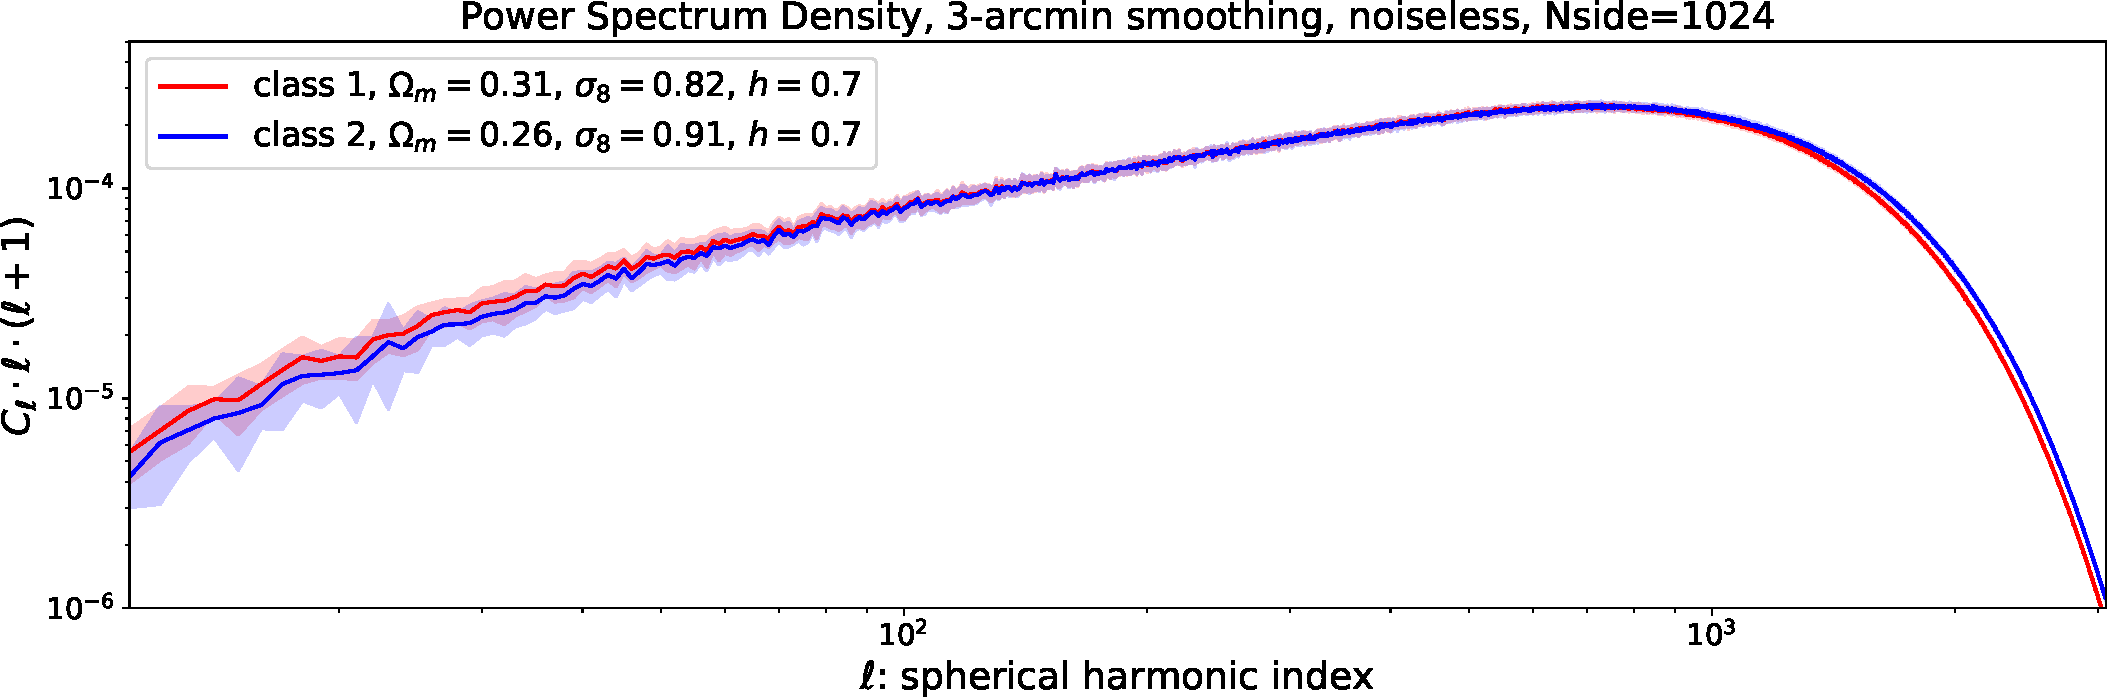
\includegraphics[width=\linewidth]{psd_sigma3}
\caption{Power spectrum densities of the noiseless maps. The maps have been smoothed with a Gaussian kernel of radius $3$ arcmins to remove high frequencies. The cosmological models could otherwise have been distinguished by looking at the PSDs.}
\label{fig:psd_sigma3}
\end{figure}

The simulations are created using the fast lightcone method described in~\citep{sgier2018fastgeneration}.
However, we use only a single simulation box, as opposed to two used in that work, as we use source galaxies at lower redshift of $z=1$, instead of $z=1.5$.
As a simulator we use \pkg{L-PICOLA} \citep{howlett2015lpicola}, a fast and approximate code for N-body simulations.
For each class, we generate $30$ simulations (both class have the same initial parameters).

Out of the $60$ simulations, $20$ are kept for the test set.
\figref{map_sample} shows the full sky simulations and a zoom region for model 1 (top) and model 2 (bottom).
Initial conditions for these simulations were the same, so the differences in structures can only be attributed to different cosmological parameters used to evolve the particle distribution.

\begin{figure*}[!ht]
\centering
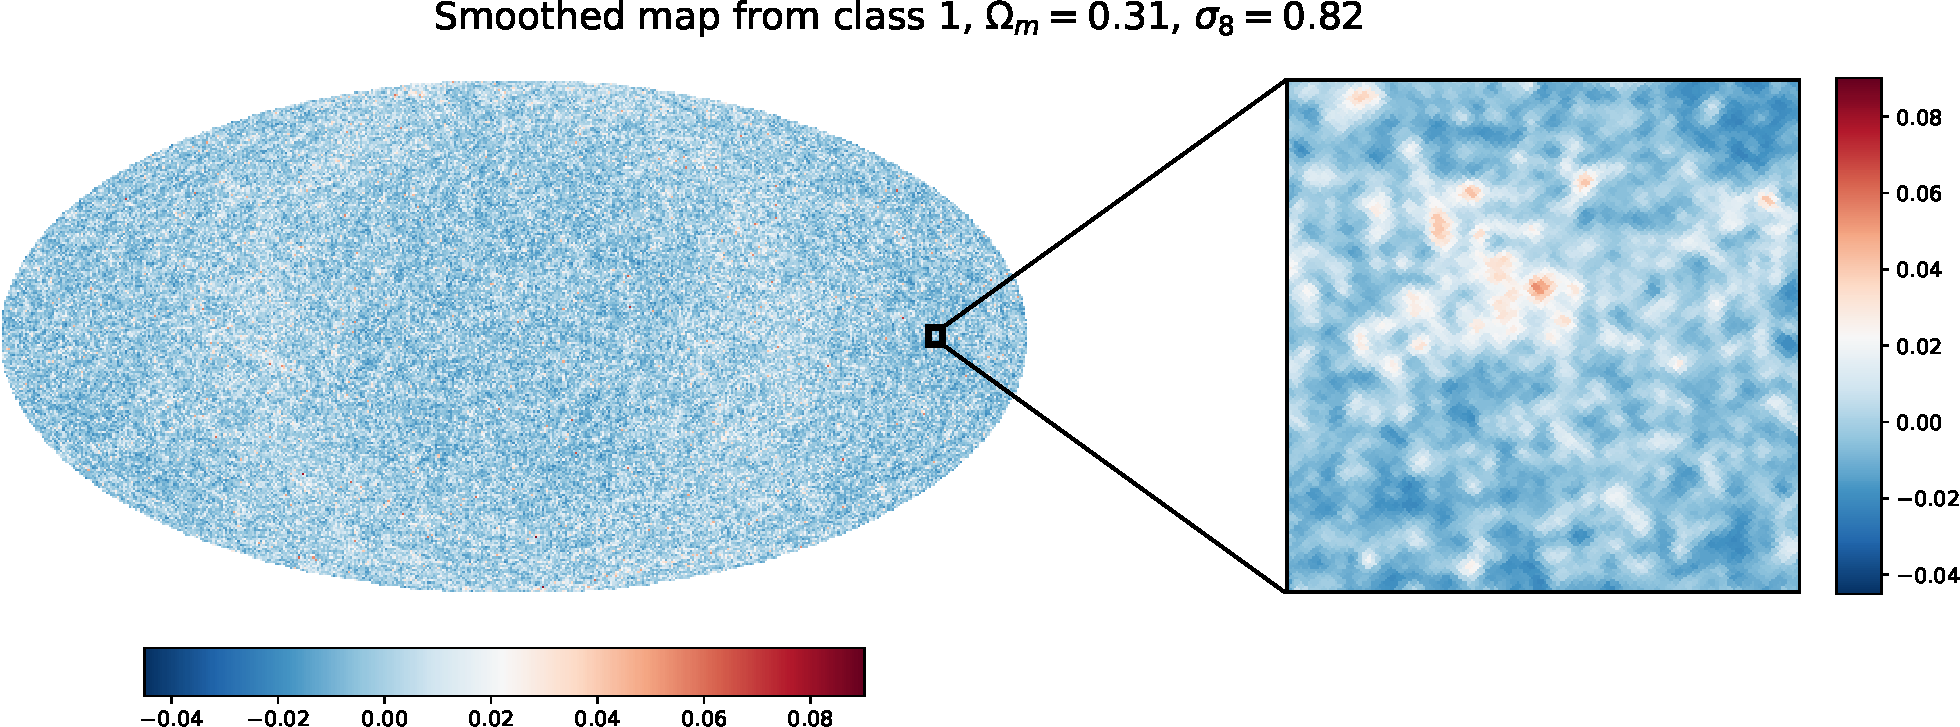
\includegraphics[width=0.48\linewidth]{smooth_map_class_1}
\hfill
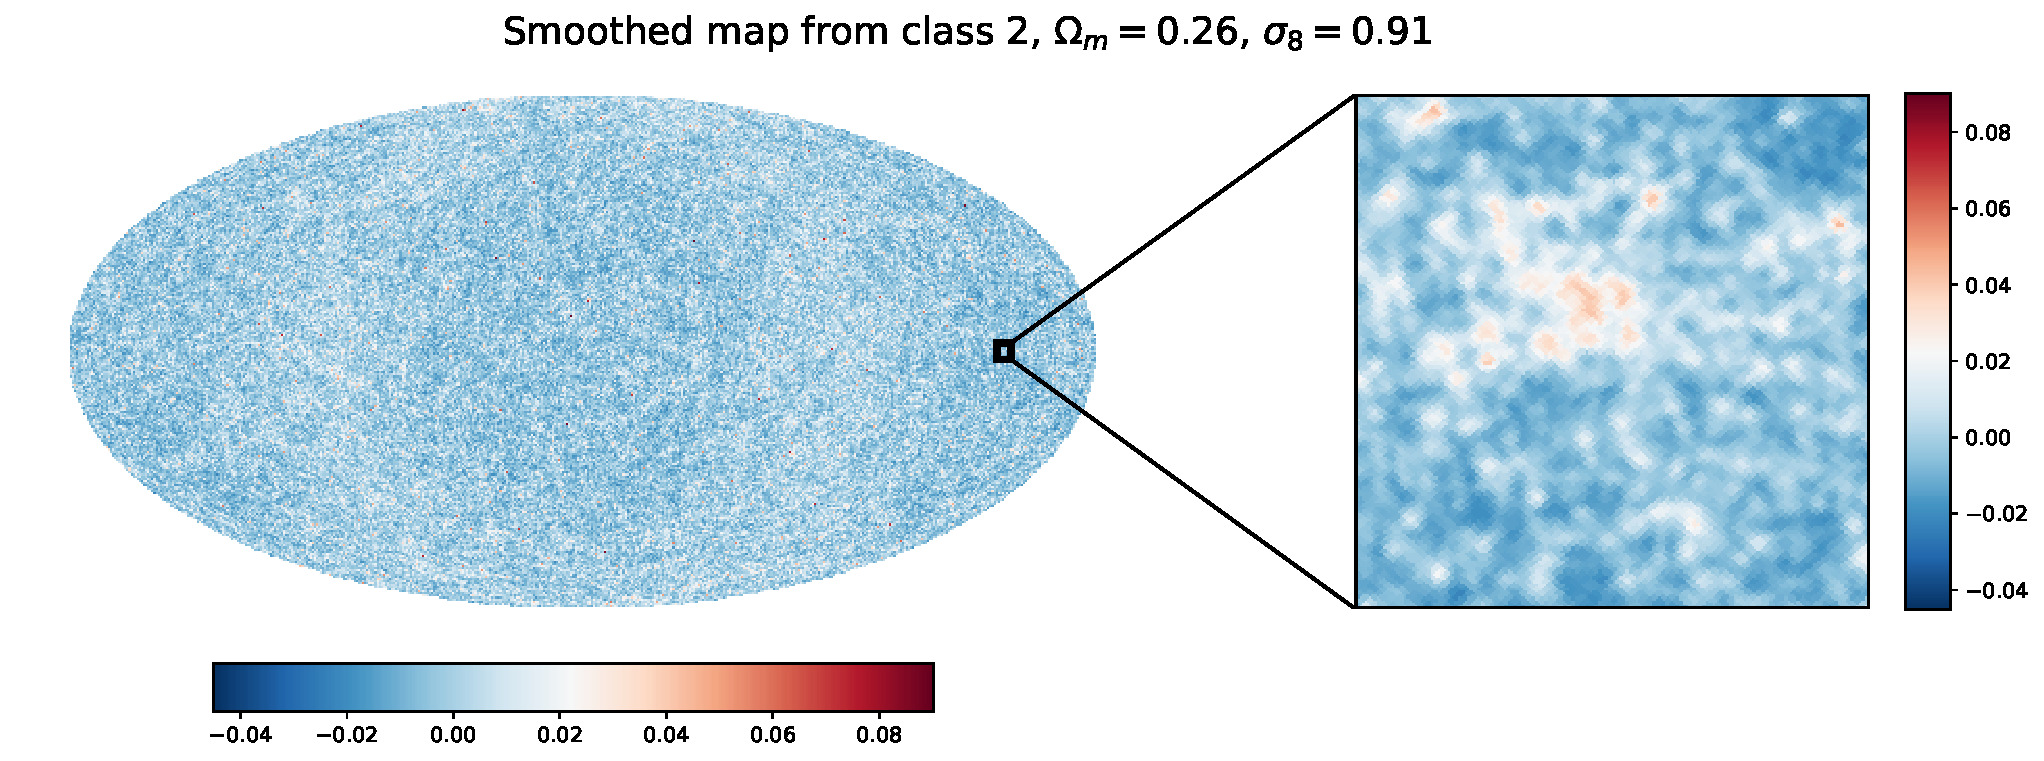
\includegraphics[width=0.48\linewidth]{smooth_map_class_2}
\caption{Example maps from two classes to be discriminated. Left: model 1 with $\Omega_m=0.31$ and $\sigma_8=0.82$. Right: model 2 with $\Omega_m=0.26$ and $\sigma_8=0.91$.
The initial conditions for both simulations were the same, so differences only arise due to different cosmological parameters. \nati{Tomek: Is this correct?}}
\label{fig:map_sample}
\end{figure*}



\subsection{Problem formulation}
While the number of maps might sound small for deep learning, the information contained in the maps is very recurrent, allowing us to use parts of the map as samples for our simulation.
Leveraging the properties of the HEALPix sampling, we can split each maps
into $12*o^2$ ($o=1,2,4,\dots$) samples that span a smaller part of the sphere.
As shown in \figref{part_sphere}, we used $o=1,2,4$ as the resulting
samples are large enough to suffer from the effects of the spherical geometry. We
decided to only report simulation results for this specific setting as spherical
cosmological data usually does not span the full sphere. Nevertheless, our code
includes an example using the full sphere.

\begin{figure}[!ht]
\centering
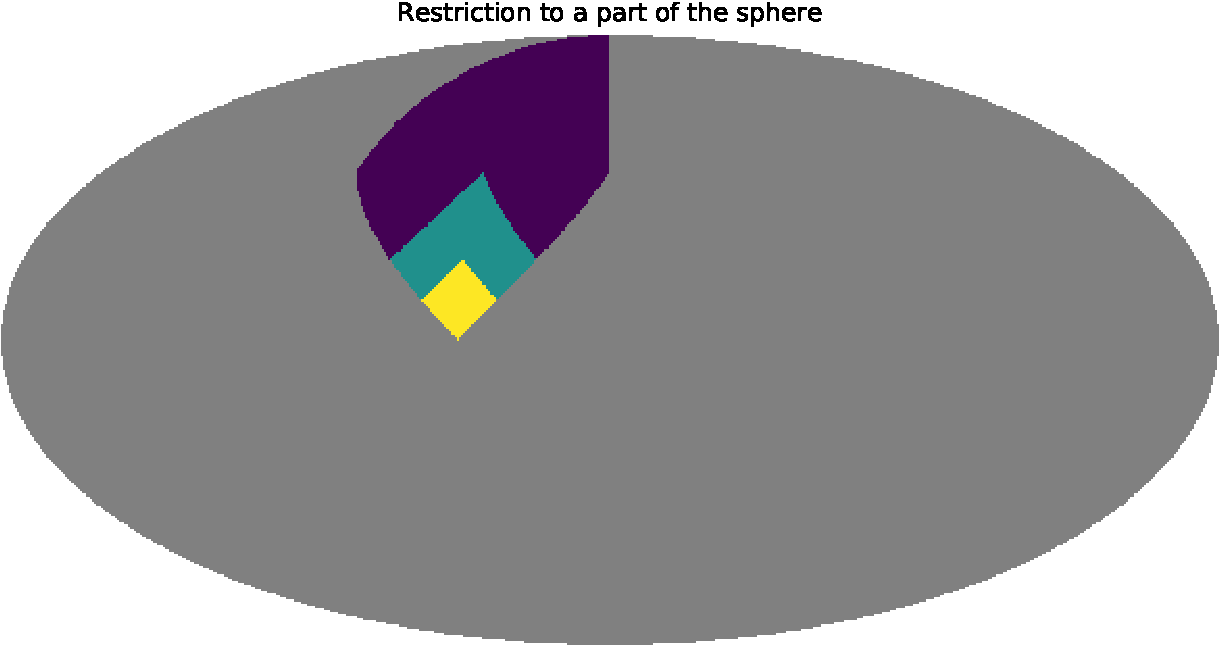
\includegraphics[width=\linewidth]{part_sphere}
\caption{Three parts of the sphere with different sizes. Blue: $o=1$. Green: order $o=2$. Yellow: order $o=4$.}
\label{fig:part_sphere}
\end{figure}

We build a robust classifier, i.e., an automatic way to
discriminate between the two classes in the presence of noise.
We check the classification performance as a function of the area used, i.e., "the order" $o$ and also as a function of the relative level of the noise added to the map.

For all the experiments, we work with centered Gaussian noise.
While the noise model is real mass maps often has a slightly different distribution, Gaussian should be a sufficient model to demonstrate the performance of our method.
To improve the stability of the spherical CNN, we slowly increase the amount of noise added to
the training data over the iterations. Furthermore in order to avoid
overfitting, the noise is randomly produced during the training process. We trained our
model between $50$ and $290$ epochs depending on the complexity and the size of
the problem. $20\%$ of the training set that we call "validation set" was left out of the training process and simply used to assess the global performance and overfitting of
the network.
Training took less than a day for each model using an NVIDIA Tesla K20.

We compare the performance of the spherical CNN against two simple benchmark
algorithms. The two baselines are based on building features with a) the Power
Spectral Densities (PSD) and b) the histogram of pixels in the maps~\cite{patton2017cosmologicalconstraints}.
After a normalization, those features are then classified use a Support Vector
Machine (SVM) with a linear kernel. Other kernels did not provide better results
while having worse scaling properties. All classifiers are trained with noisy samples. For fairness, we augmented the dataset
of the baseline algorithm in a similar way as for the network, i.e, with
created an "unlimited" number of samples by adding new random realizations of
the noise. We stop adding new samples in the classifier once the validation
error converge to a value. This process is detailed in Appendix~\ref{sec:dataset_augmentation}. We tuned the parameter using cross-validation with the validation set.

\subsection{Results}

We present in \figref{results} the results for 5 different noise
levels and $3$ different sample areas. The spherical CNN has a significant lead for all levels of noise and sample areas.
In particular, the difference seems to increase as the problem becomes more complex, i.e., as the order is increased and there is less information in each sample.
This is likely due to the fact that the SCNN can learn optimal features for the problem and do not rely on our humanly limited feature design.

We observe that the PSD features, i.e.,
one of the most used techniques for model discrimination in cosmology, is unable
to perform the desired task. The main reason is that the two different models
have very similar PSDs (see \figref{psd_sigma3}). As a result, one
needs to use other statistics to solve the problem. In this case, the
histogram features that have been built for the problem allow for a significant improvement over the PSD ones.
Unfortunately, while the histogram features contain information about the
distribution of pixels, they do not include any spatial information. In
contrast, both the PSD features and the SCNN can exploit the spatial
information.
Note that without this graph structure, a fully connected neural network approach would have to be used. Problematically, fully connected neural networks do not scale well with the number of pixels.




\begin{figure*}[!ht]
\centering
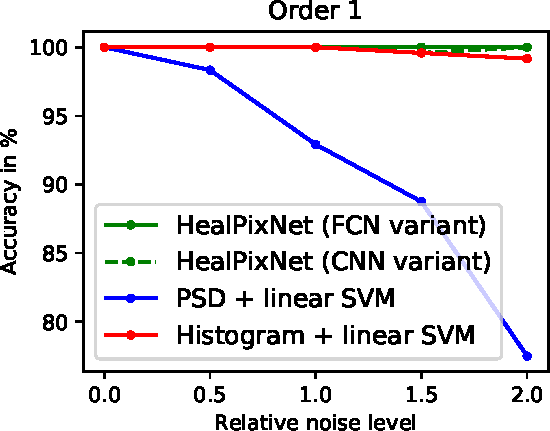
\includegraphics[width=0.32\linewidth]{result_order1}
\hfill
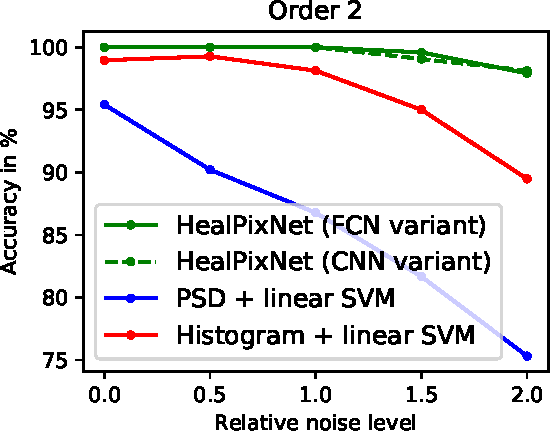
\includegraphics[width=0.32\linewidth]{result_order2}
\hfill
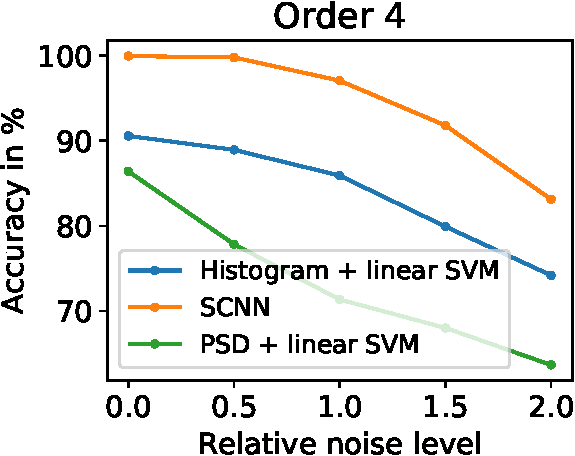
\includegraphics[width=0.32\linewidth]{result_order4}
\caption{Classification errors for the 3 different problems.}
\label{fig:results}
\end{figure*}


\subsection{Filter visualization}
One common visualization for CNN is to observe the shape of the learned filters.
Since our construction leads to almost (up to the sampling irregularities)
spherical filters, we plot in \figref{learned_filter} both the section (on the
sphere) and a gnomonic projection on a plane of a random selection of learned
filters. The filters are selected from the last layer of the network
corresponding the experiment with order $o=2$ for a relative noise level of
$2$. Nevertheless, all networks presented similar gnomonic and section pattern, at least from a
human perspective. The gnomonic projection clearly exibits the sampling issue
of HEALPix.
For a detail, on how the convolution kernels are plotted, please refer to Appendix~\ref{sec:filter_visualization}.
While it is usually difficult to interpret the shape of the filters in the context of the type of data, we can notice that they often have a ``peak'' like structures.
An example of filter interpretation was demonstrated in \citep{Ribli2018learningfrom}.
% \todo{Tomek: can you say something about the filters.}
% \TK{Done }

\begin{figure*}[!ht]
\centering
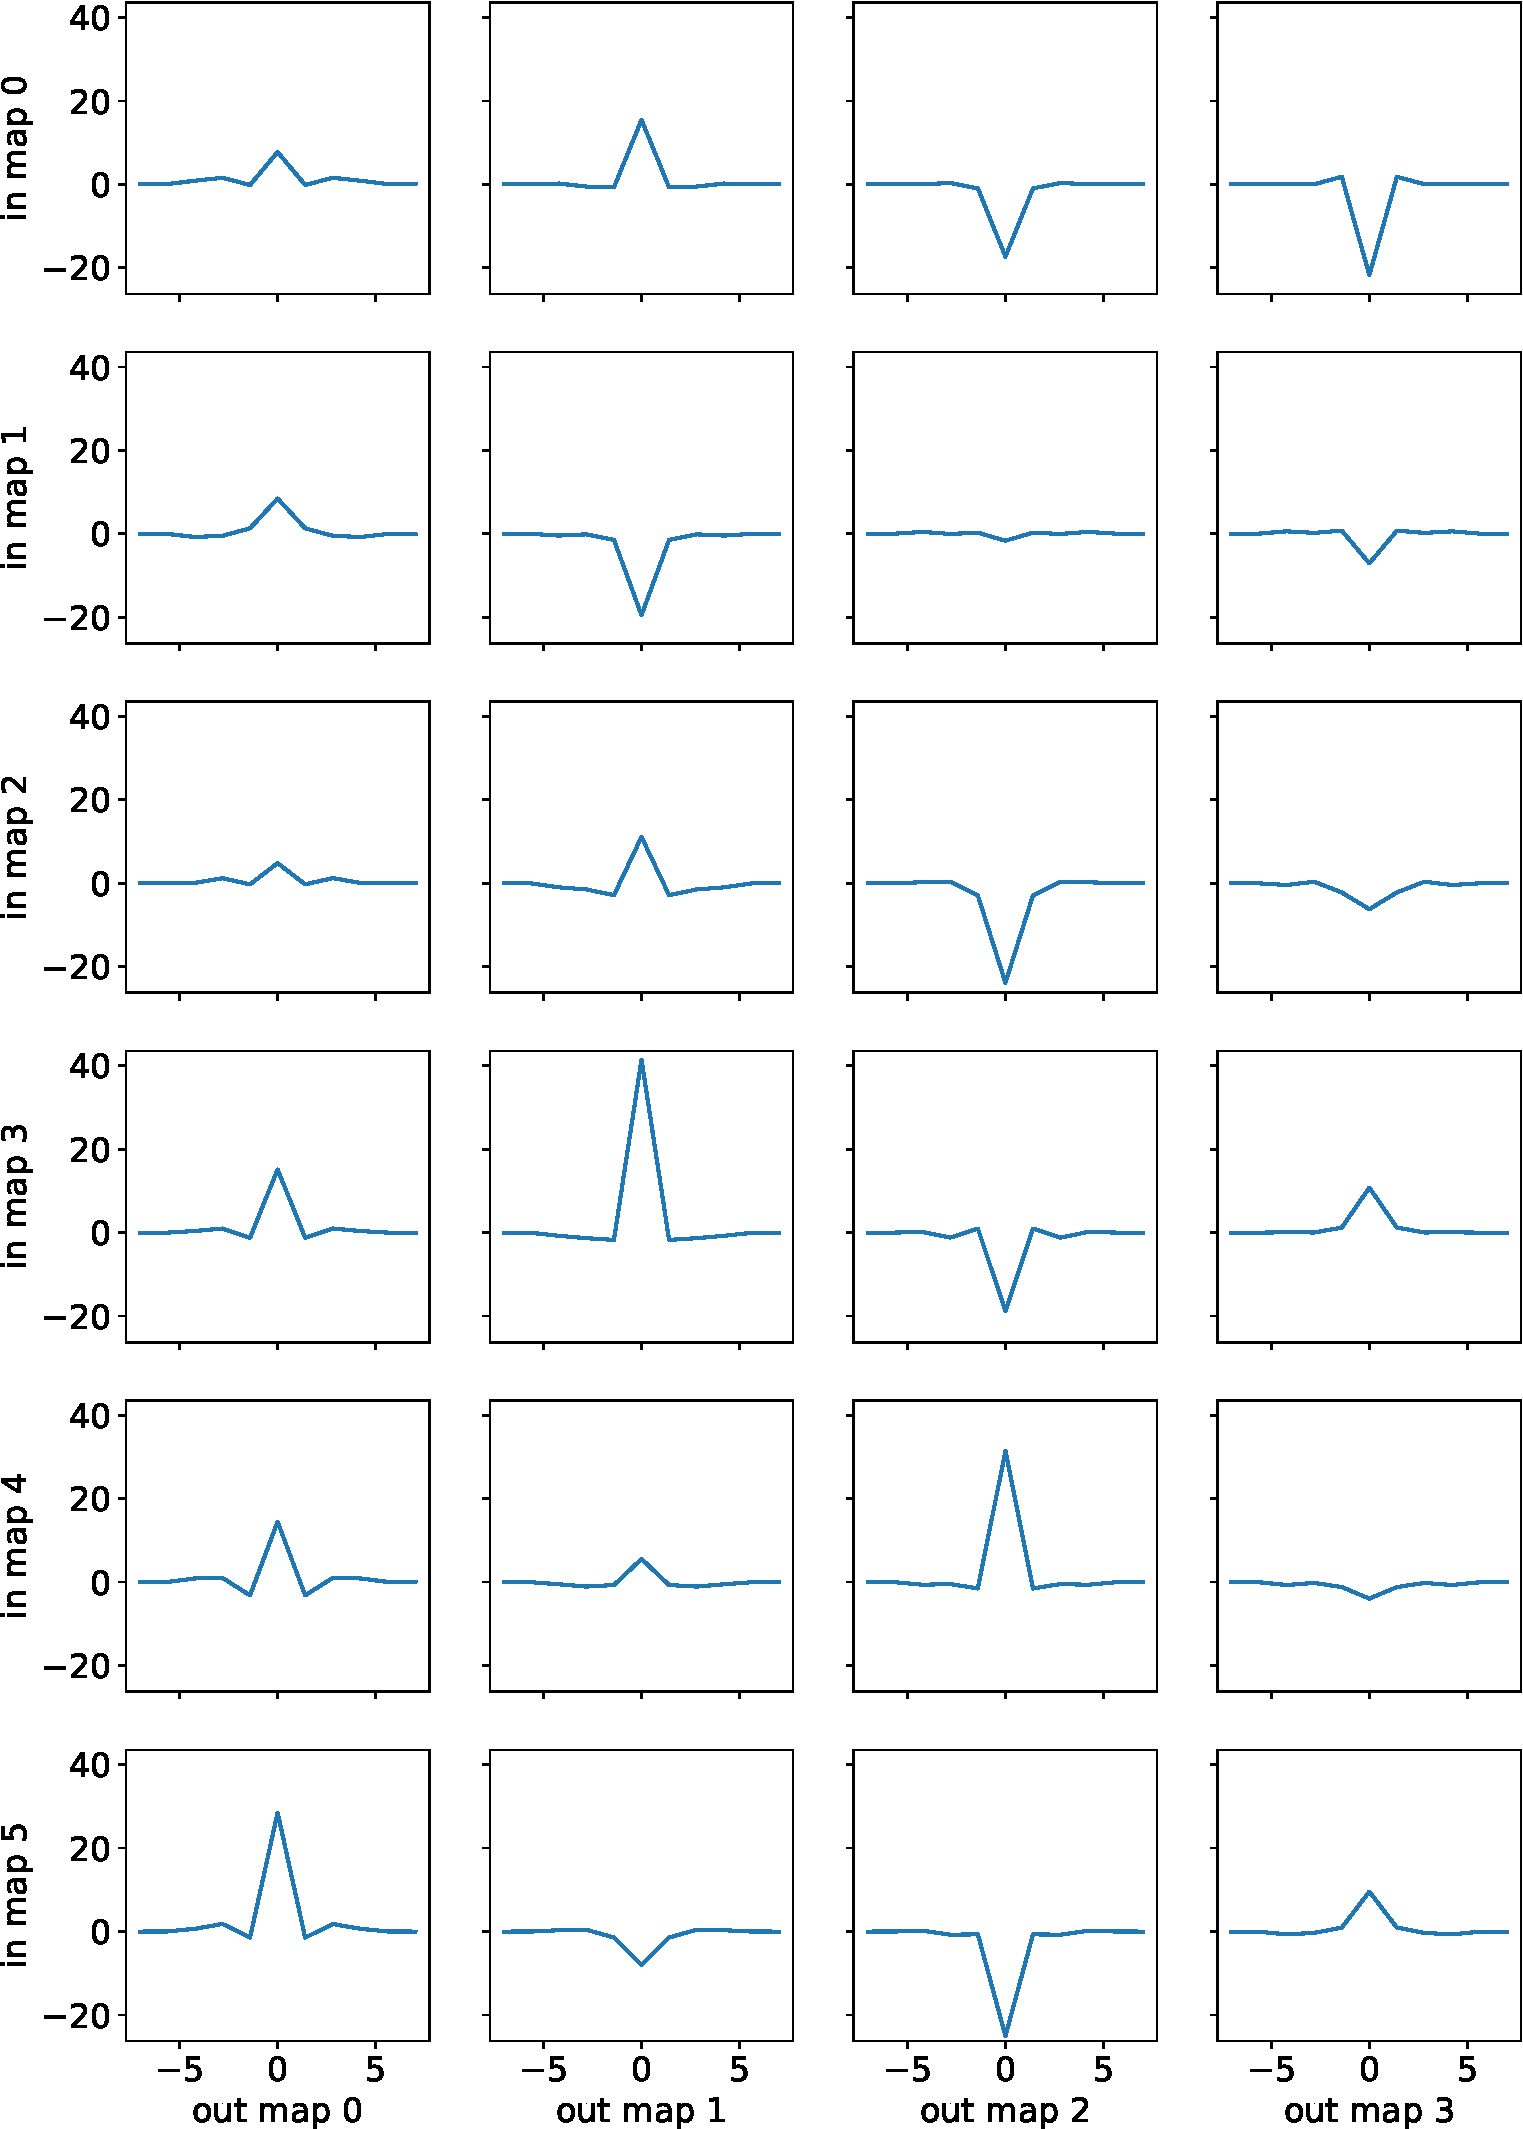
\includegraphics[width=0.47\linewidth]{section_filter_last}
\hfill
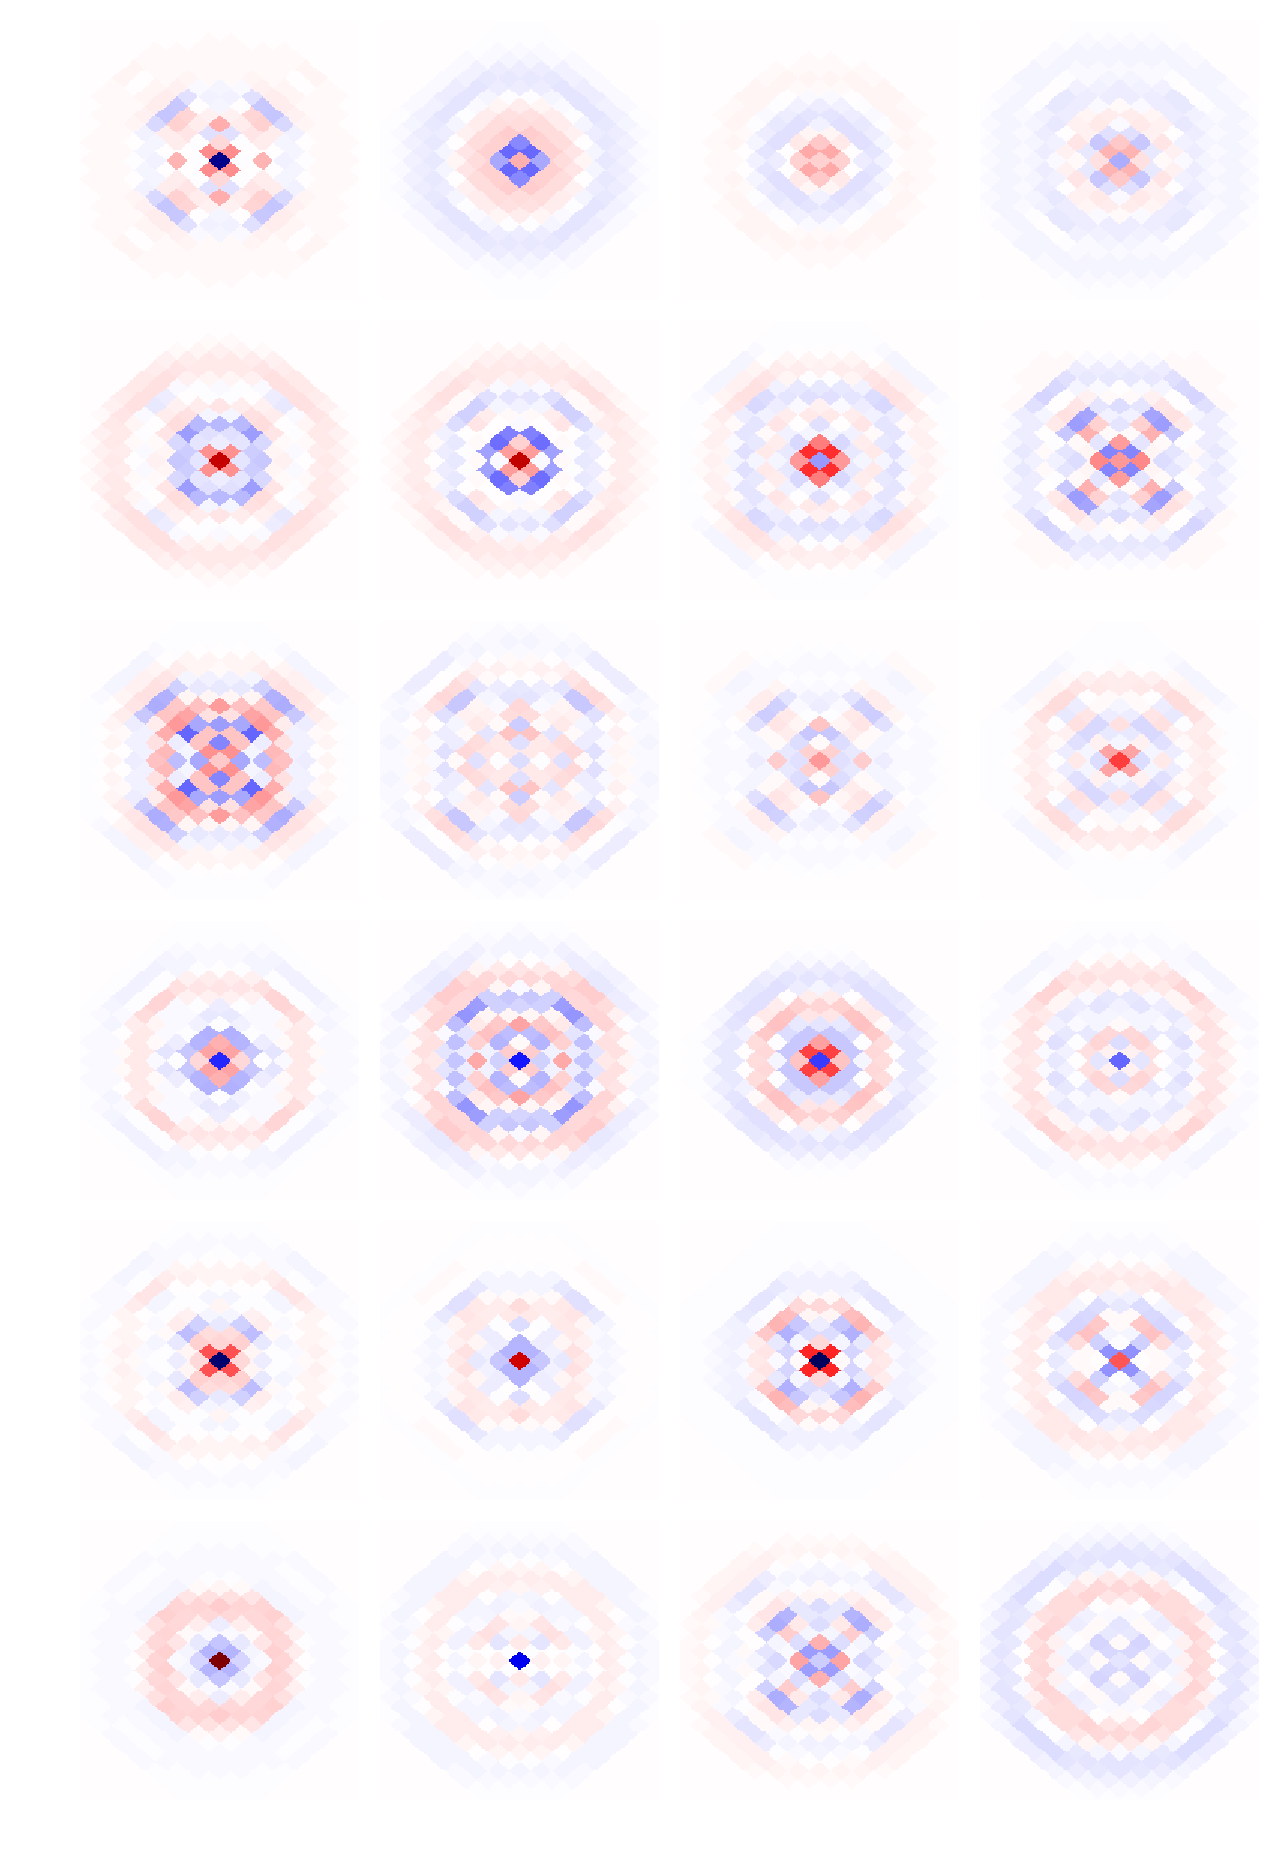
\includegraphics[width=0.45\linewidth]{gnonomic_filter_last}
\caption{24 learned filters selected from the last spherical convolutional layer. Left: section. Right: gnonomic view.}
\label{fig:learned_filter}
\end{figure*}

\section{Discussion}

Because of the spherical domain, the method presented here restricts the shape of the filters learned by the network to be radial.
While this may be a less general design compared to the one used by conventional CNNs on flat images, we found it to still work efficiently for our test cases.
The layered structure of the network can partially compensate for that.
Further generalizations to non-radial filters may be possible [cite?], but we leave it to future work.

\nati{Should the discussion be merged with the result section?}

\section{Conclusion}
\label{sec:conclusion}

In this contribution, we presented HealpixNet, a spherical CNN for the HEALPix sampling. The gist of our construction resides in using a graph to model the sphere.
This allows us to leverage the advantages of the graph convolution, i.e., it is both efficient (with a complexity of $\mathcal{O}(N_{pix})$) and flexible (allow to work only on a part of the sphere) while it still captures well the spherical properties of the domain.
We also show on a range of classification problems that the neural network systematically significantly outperform classical methods.

As shown in this contribution, modelling the discretized sphere, a 2D manifold in $\R^3$, by a graph enables an efficient convolution operation on any pixelization. Hence, it relaxes the iso-latitude constraint on sampling schemes who aim to enable fast convolutions. For applications which can tolerate small imprecisions in rotation invariance --- the fact that the action of a graph filter slightly depends on the location --- this relaxation might enable researchers to consider sampling sets with different properties.

The main product of this contribution is HealpixNet,\footnote{\url{https://github.com/SwissDataScienceCenter/HealpixNet}} a small and easy-to-use python package for cosmologists to classify sky maps.
As a future work, we intend to (i) further investigate the link between the graph Fourier basis and the spherical harmonic and (ii) compare HealpixNet to other spherical CNN using different sampling schemes.

\section*{Thanks}

%% The Appendices part is started with the command \appendix;
%% appendix sections are then done as normal sections
\appendix

\section{Graph Fourier modes and spherical harmonics}
\label{sec:comparison_spherical_harmonics}
\label{sec:border_effects}

The eigenvalues of the graph Laplacian $\L$, shown in \figref{graph_eigenvalues}, are clearly organized in frequency groups of $2\ell + 1$ orders for each degree $\ell$.
The first 16 eigenvectors $[\b u_1, \ldots, \b u_{16}]$ of the graph Laplacian $\L$, forming the lower part of the graph Fourier basis $\U$, are shown in \figref{graph_harmonics}. \figref{subspace_harmonics_eigenvectors} shows the correspondence between the subspaces spanned by the graph Fourier modes and the spherical harmonics. While there is again a clear resemblance with the spherical harmonics, the small irregularities in the sampling (non-constant number of neighboring pixels and varying distance between pixels, see \figref{healpix_graph_4}) have an effect on the graph Fourier modes.
First, counter-intuitively, some eigenvectors will be localized~\citep{perraudin2018global}, i.e, they will span a small part of the sphere.
Second, as the resolution is increased with $N_{side} \rightarrow \infty$ and $N_{pix} \rightarrow \infty$, we are still unsure if the eigenvectors would converge towards the spherical harmonics. We believe that it might be the case for a different construction of the graph (fully connected) and that a proof could be built on top of the work of~\cite{belkin2007convergence}. That is however out of the scope of this contribution.

\begin{figure}
	\centering
	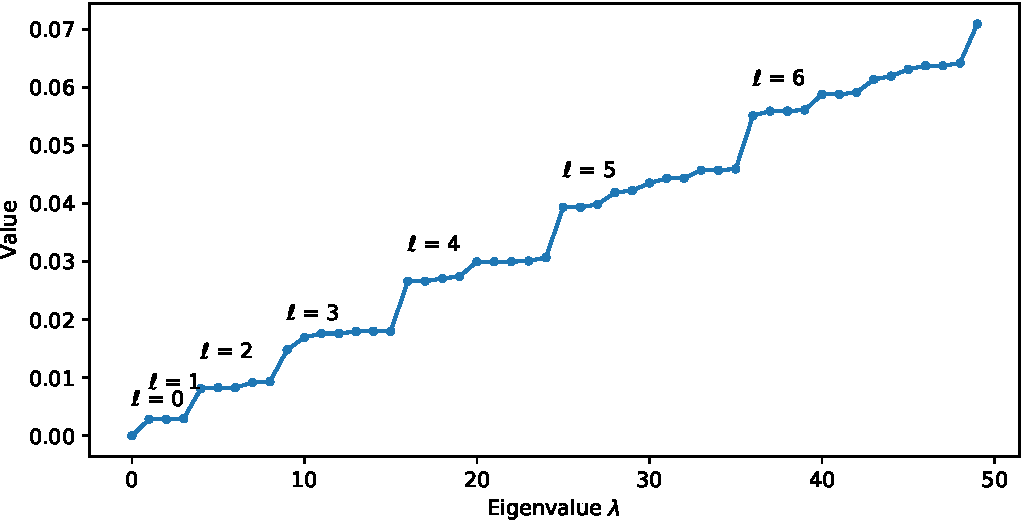
\includegraphics[width=\linewidth]{graph_eigenvalues}
	\caption{The eigenvalues $\bLambda$ of the graph Laplacian $\L = \U \bLambda \U\trans$, which corresponds to squared frequencies, are clearly organized in groups. Each group corresponds to a degree $\ell$ of the spherical harmonics. Each degree has $2\ell + 1$ orders. See also \figref{graph_harmonics}.}
	\label{fig:graph_eigenvalues}
\end{figure}

\begin{figure}
	\centering
	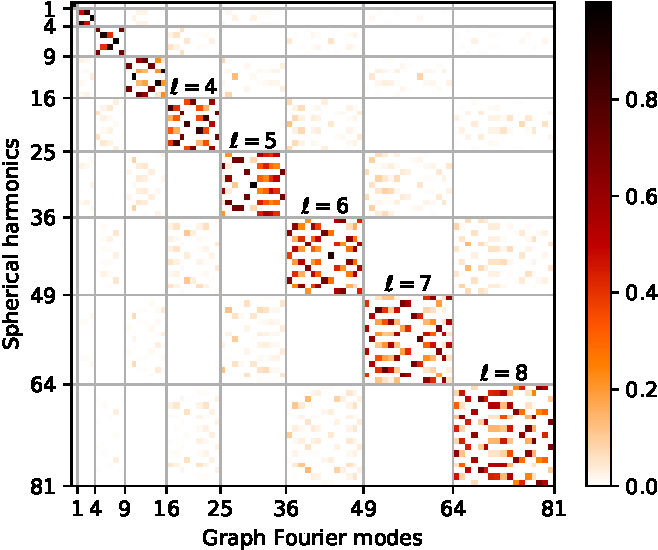
\includegraphics[width=\linewidth]{subspace_harmonics_eigenvectors}
	\caption{Correspondence between the subspaces spanned by the graph Fourier modes and the spherical harmonics. Each pixel on the plot is the dot product between one spherical harmonic and one graph Fourier mode $\b u_i$. The plot clearly shows how the subspaces are aligned: modes and harmonics which correspond to different degrees $\ell$ are mostly orthogonal to each other, while modes and harmonics which correspond to the same degree $\ell$ are linearly dependent. There is $2 \ell + 1$ orders per degree $\ell$. Moreover, we see that the Fourier modes have the correct symmetries, indicated by the perfect orthogonality between even and odd functions.}
	\label{fig:subspace_harmonics_eigenvectors}
\end{figure}

The graph setting used through this contribution assumes reflective border conditions. That is irrelevant when working on the complete sphere as this surface has no border. When working with a part of the sphere however, its border slightly affects the convolution. As depicted in \figref{border_effects}, a filter localized near the border of a part of the sphere (via $h(\L) \b \delta_i$) no longer has an isotropic profile. These border effects can however be mitigated by padding with zeros a small area around the part of interest.

\begin{figure}[!ht]
	\centering
	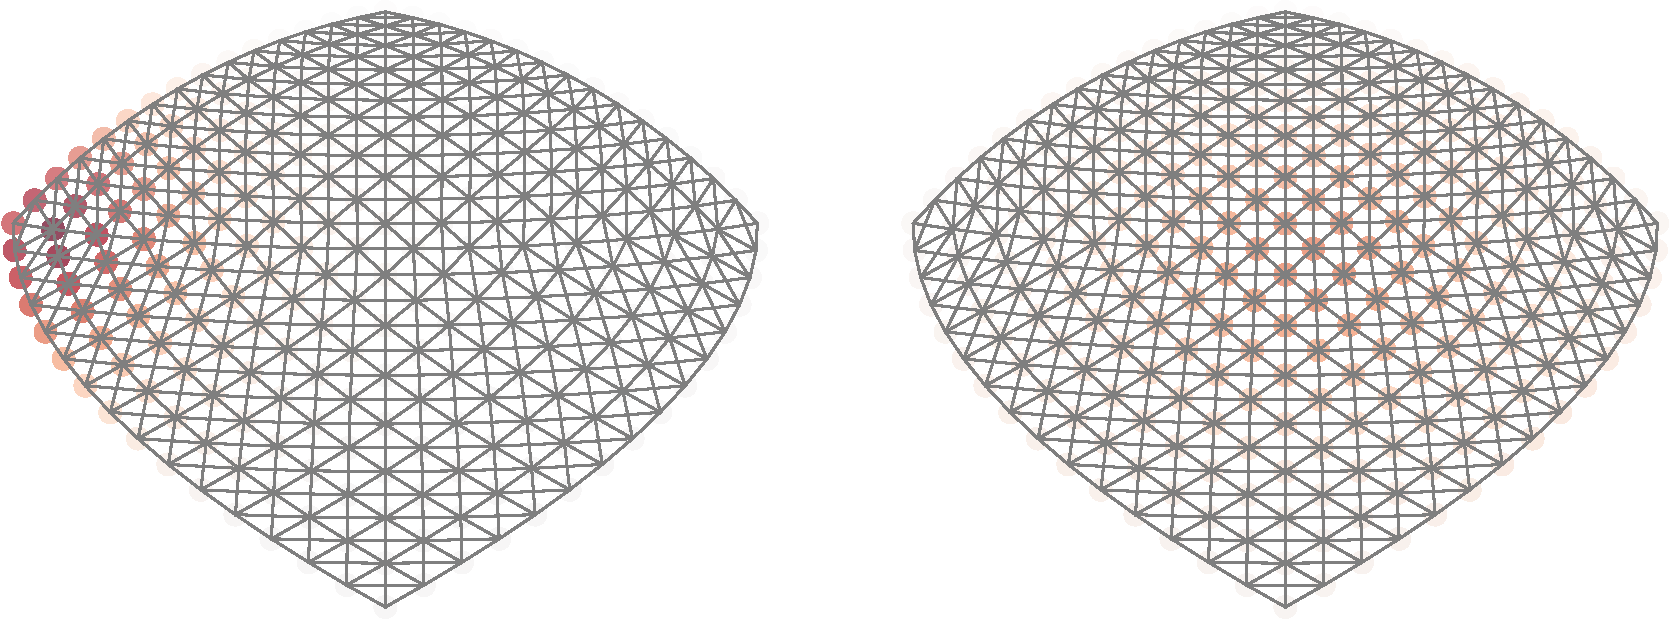
\includegraphics[width=\linewidth]{border_effects}
	\caption{Convolution kernel (also called filter) $h$ localized in the center and left corner of a surface. A filter is localized on pixel $i$ as $h(\L) \b \delta_i$ (see \secref{graph_convolution} and \eqnref{graph_convolution_spatial}). The graph is built from $1/12^\text{th}$ of the sphere at $N_{side} = 16$. The filter is not isotropic anymore when localized on the left corner due to border effects. The graph representation of a manifold assumes reflective border conditions.}
	\label{fig:border_effects}
\end{figure}

\section{Filter visualization}
\label{sec:filter_visualization}

In \figref{gaussian_filters_visualization}, we present three different
visualization for a HEALPix graph convolution kernel. The kernel used is defined in the graph spectral domain as $K_t(x)=e^{-\tau t x}$. This is the domain used for our first visualization. In this case, we simply evaluate $K_t$
at the graph eigenvalues $\text{diag}(\bLambda)$. The lower eigenvalues $\lambda$ correspond to the lower frequencies, i.e., the spectral mode with less variation.
As a second visualization, we can observe the kernel directly on the sphere. To do so, we perform the convolution of a
Kroneker on the sphere plot the result with gnomonic projection. Eventually, as we are
working on the sphere with theoretically spherical filters (up to the irregularities of the sampling), we could only plot the section of the convoluted Kroneker. To do so, we convolve a Kroneker on the equator and use the equator for our section as shown in~\figref{index_section}. Note that, because of the small irregularities in the HEALPix
sampling, the second and the third methods are subject to small variations depending on the
chosen Kroneker.

\begin{figure*}[!ht]
\centering
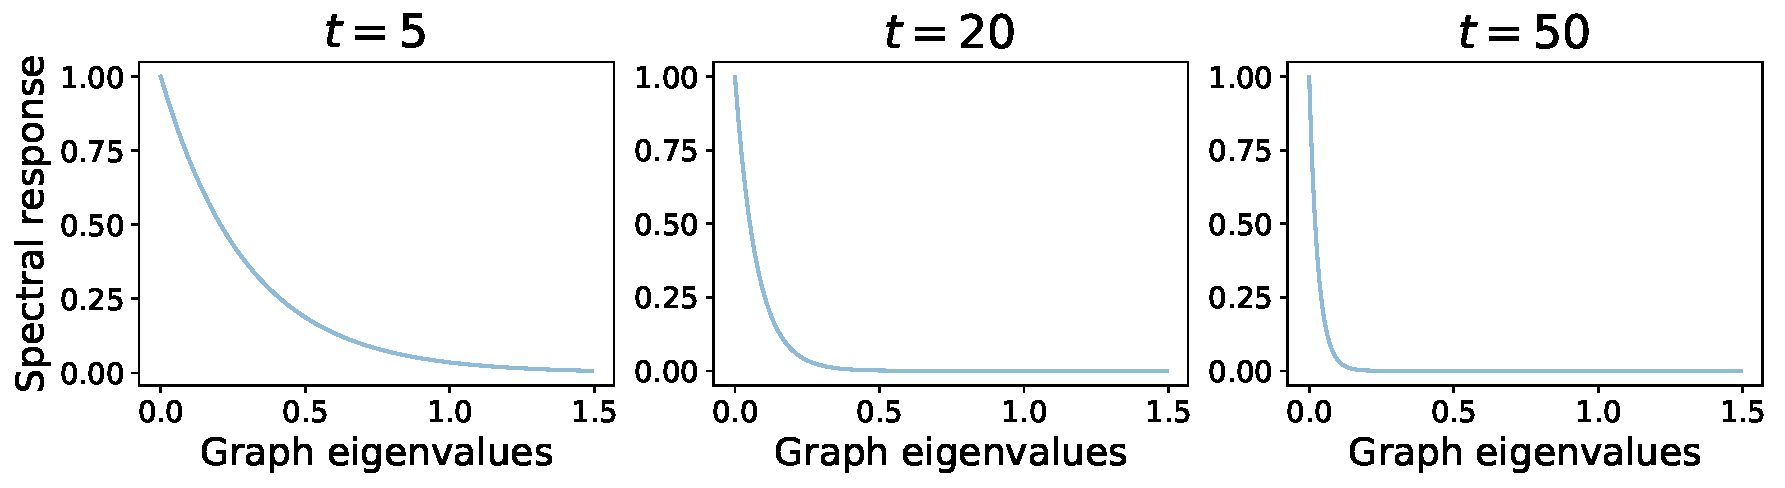
\includegraphics[width=\linewidth]{gaussian_filters_spectral}
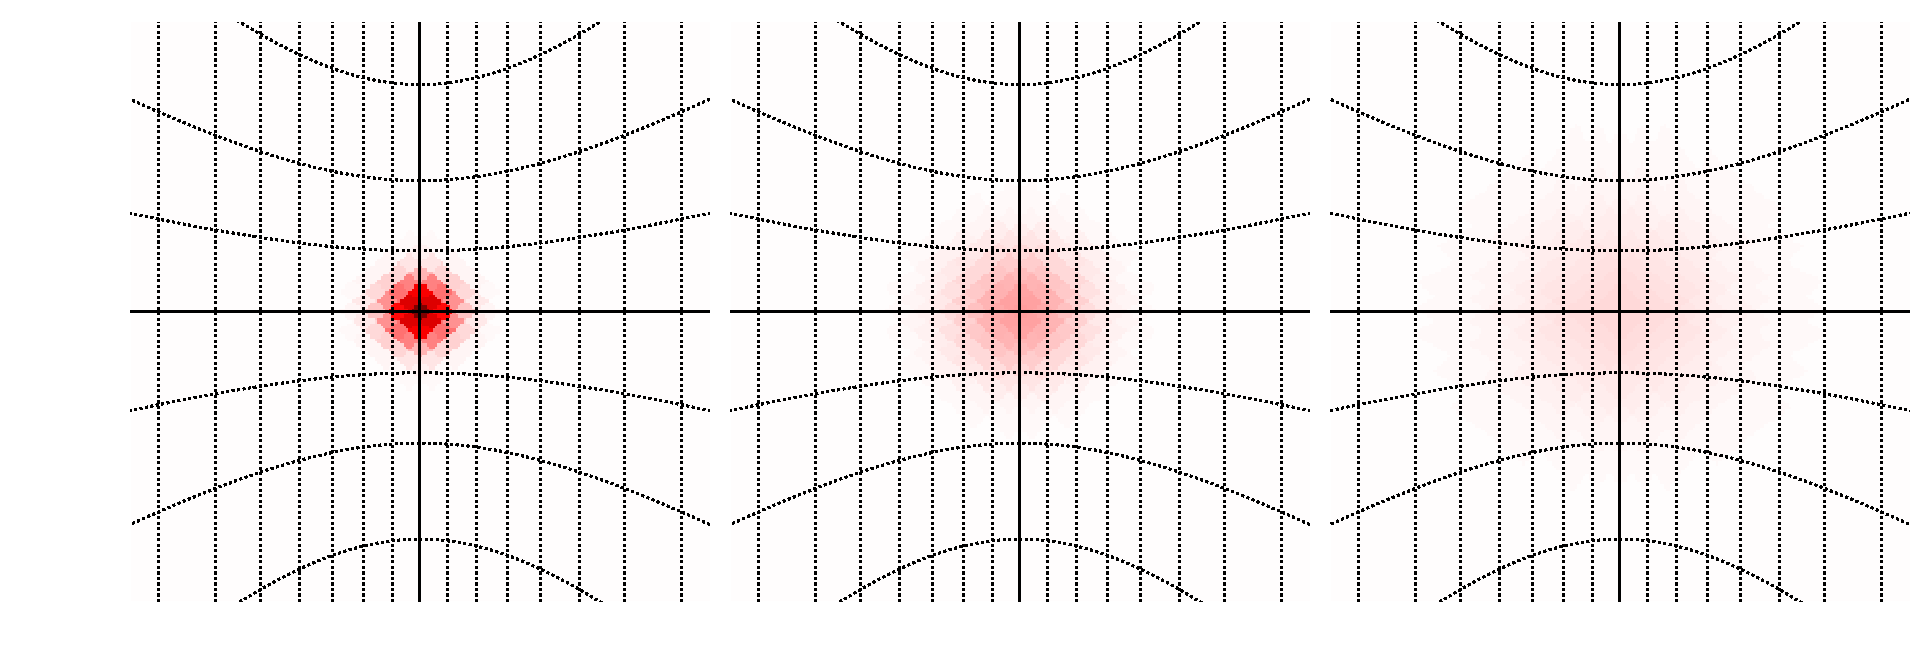
\includegraphics[width=\linewidth]{gaussian_filters_gnomonic}
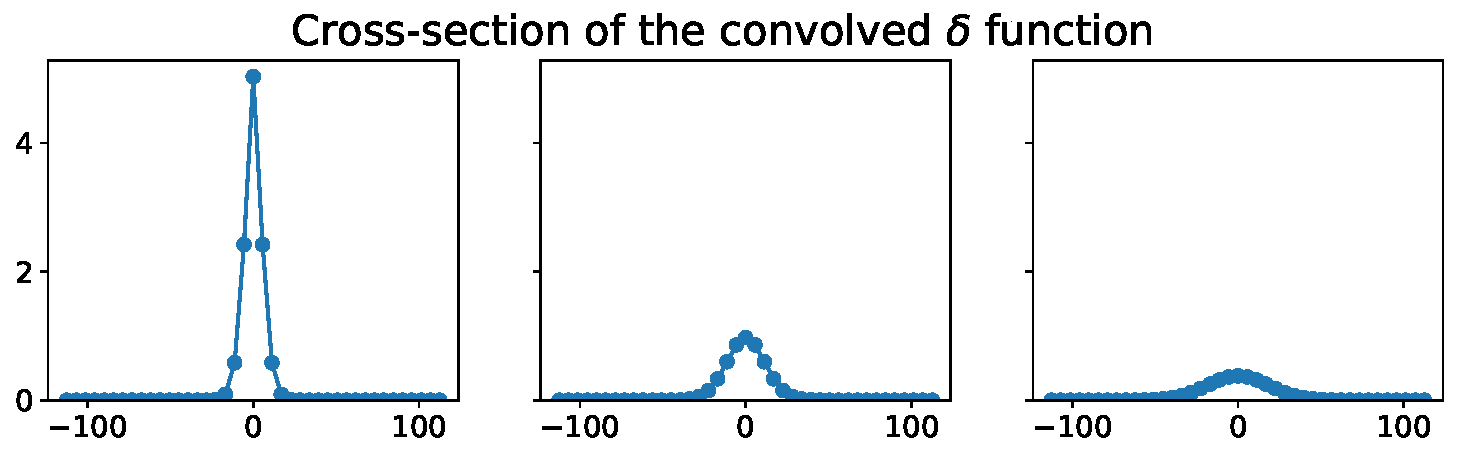
\includegraphics[width=\linewidth]{gaussian_filters_section}
\caption{Three different visualizations of the convolution kernel $K_t(x)=e^{-\tau t x}$.
Top: graph spectral domain.
Middle: gnomonic projection.
Bottom: section plot.}
\label{fig:gaussian_filters_visualization}
\end{figure*}

\begin{figure}[!ht]
\centering
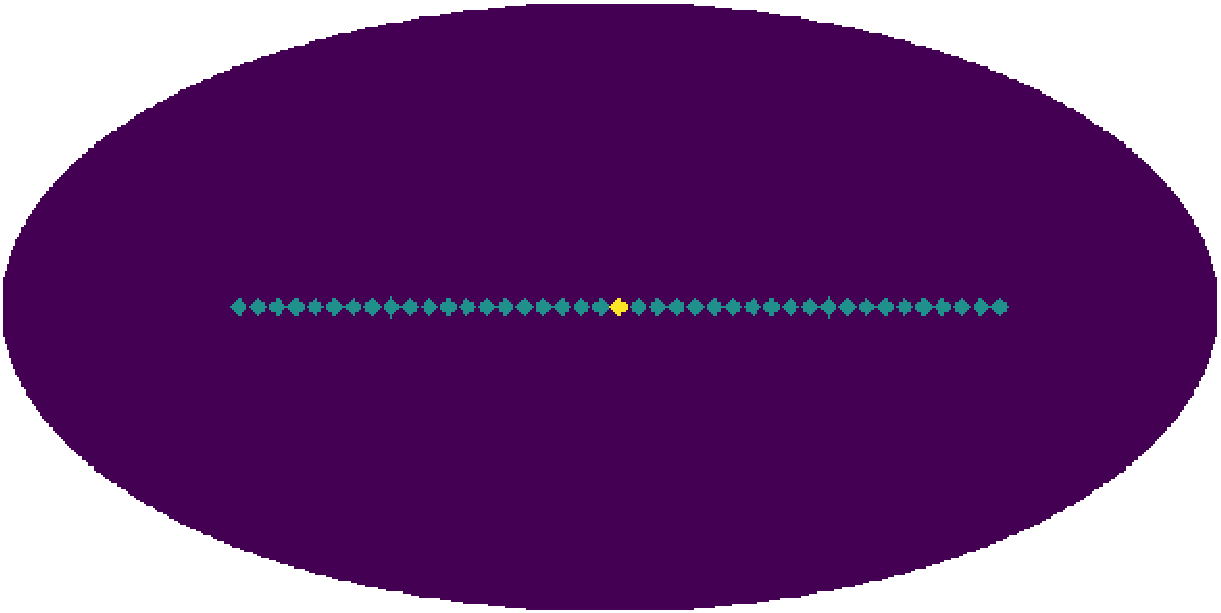
\includegraphics[width=0.6\linewidth]{index_plotting_order20_nside16}
\caption{Indexes selected for the section ploting of \figref{gaussian_filters_visualization} middle. The delta was placed on the yellow node.}
\label{fig:index_section}
\end{figure}

\section{Augmentation of the dataset for the SVM classifier}
\label{sec:dataset_augmentation} The original number of samples $480$, $1920$,
$7680$ respectively for order $o=1,2,4$ is considered rather low for usual
deep learning technique, especially when one desire to build a noise robust
classifier. As a result, we use a classical dataset augmentation technique.
Before entering the network for training each sample is added a random
realization of Gaussian noise. The effect is twofold. First, the network never
ends up seing the same sample and is less likely to overfit the training set.
Second the trained network will be robust to Gaussian noise.

When comparing the network, we want to ensure that the SVM classifier has
access to the same amount of data that the network, i.e, potentially an
infinite number of samples. Hence, we fit different linear SVM classifier using
various training set size until we observe experimentally that
increasing the amount of data does not improve the classifier. The validation
set remain the same and is used for cross-validation to tune the L2
penalization parameter of SVM. Eventually, we evaluate the final classifier on
the testing set. An example of the evolution of the training and valdication
error is shown in \figref{hist_error_evolution}.

\begin{figure}[!ht]
\centering
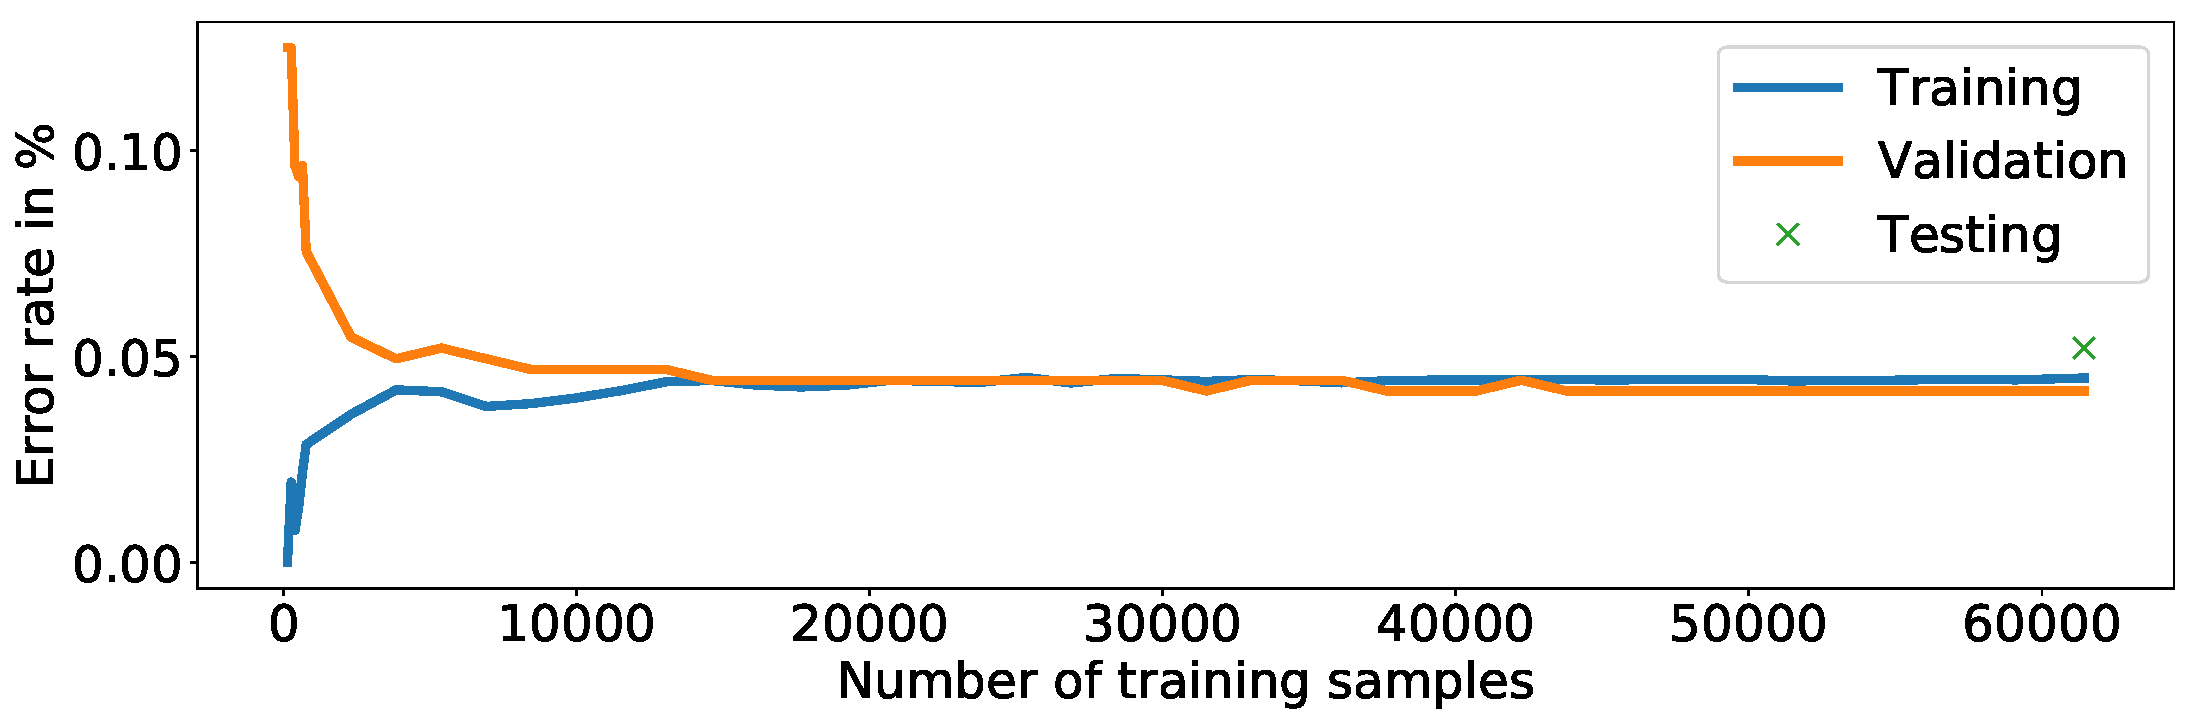
\includegraphics[width=\linewidth]{hist_error_order2_noise1_5}
\caption{Evolution curve of the error with respect to the number of training samples for histogram features and a linear classifier (setting: order 2, relative noise level: 1.5). The validation error might be slightly below the training error because we use it for cross-validation.}
\label{fig:hist_error_evolution}
\end{figure}

%% If you have bibdatabase file and want bibtex to generate the
%% bibitems, please use
%%
\section*{Bibliography}
\bibliographystyle{elsarticle-harv}
\bibliography{biblio}

\end{document}

\endinput
%%
%% End of file `elsarticle-template-harv.tex'.
